\documentclass[12pt,UTF8]{ctexbook}
\usepackage{ctex}
\usepackage{caption}
\usepackage{polynom}
\usepackage{graphicx}
\usepackage{float}
\usepackage{wrapfig}
\usepackage{array}
\usepackage[table, dvipsnames, svgnames, x11names]{xcolor}
\usepackage{colortbl}% 
\usepackage{tabularx}
\usepackage{amsmath}
\usepackage{amssymb}
\usepackage{xfrac}
\usepackage{eucal}
\usepackage{titlesec}
\usepackage{amsthm}
\usepackage{tikz-cd}
\usepackage{enumitem}
\usepackage{verbatim}
\usepackage{fontspec,xunicode,xltxtra}
\usepackage{xeCJK} 
\usepackage{tikz}

% 修改脚注的编号为加圈样式,并且各页单独编号
\usepackage{pifont}
\usepackage[perpage,symbol*]{footmisc}
\DefineFNsymbols{circled}{{\ding{192}}{\ding{193}}{\ding{194}}
{\ding{195}}{\ding{196}}{\ding{197}}{\ding{198}}{\ding{199}}{\ding{200}}{\ding{201}}}
\setfnsymbol{circled}

\definecolor{gl}{RGB}{246, 252, 240}
\definecolor{gd}{RGB}{236, 244, 230}
\definecolor{bg}{RGB}{242, 244, 228}


\setCJKmainfont[BoldFont=STZhongsong]{STSong}
\setCJKmonofont{simkai.ttf} % for \texttt
\setCJKsansfont{simfang.ttf} % for \textsf
\setlength\parskip{8pt}
\setlength{\fboxsep}{12pt}
\renewcommand\thesection{\arabic{chapter}.\arabic{section}}
\theoremstyle{definition}
\newtheorem{df}{定义}[section] 
\newtheorem*{po}{公理}
\newtheorem{pp}{命题}[section]
\newtheorem{tm}{定理}[section]
\newtheorem{cor}{推论}[pp]
\newtheorem{ex}{例子}[section]
\newtheorem{et}{例题}[section]
\newtheorem*{so}{解答}
\theoremstyle{plain}
\newtheorem{sk}{思考}[section]
\newtheorem{xt}{习题}[section]
% \newenvironment{proof2}{\paragraph{\textbf{证明:}}}{\hfill$\square$}
\renewenvironment{proof}{\paragraph{\textbf{证明:}}}{\hfill$\square$}
\renewcommand{\proofname}{\indent\bf 证明}
\renewcommand{\qedsymbol}{\hfill$\square$}
% 列举环境的行间距
\setenumerate[1]{itemsep=0pt,partopsep=0pt,parsep=0pt,topsep=0pt}
\setitemize[1]{itemsep=0pt,partopsep=0pt,parsep=0pt,topsep=0pt}
\setdescription{itemsep=0pt,partopsep=0pt,parsep=0pt,topsep=0pt}
\setlength{\intextsep}{2pt}%
\setlength{\columnsep}{2pt}%
% 新函数
\renewcommand\parallel{\mathrel{/\mskip-4mu/}}
\newcommand\parasbx{%
    \mathord{\text{%
        \tikz[baseline] \draw (0,.1ex) -- (.8em,.1ex) -- (1em,1.6ex) -- (.2em,1.6ex) -- cycle;}}}
% 章节字体大小
\titleformat{\section}{\zihao{-2}\bfseries}{ \thesection }{16pt}{}
% 封面
\title{\zihao{0} \bfseries 第四册}
\author{\zihao{2} \texttt{大青花鱼}}
% \date{\bfseries\today}
\date{}
% 正文
\begin{document}
\maketitle
\tableofcontents
\newpage

\chapter{四边形}
四边形是生活中常见的形状。下面来看几种常见的四边形。
\section{平行四边形}

\textbf{平行四边形}是一种重要的四边形。它由两组平行线确定。

设直线$l_1 \parallel l_2$,$m_1 \parallel m_2$,且$l_1$和$m_1$有交点$A$,
那么$l_2$和$m_1$、$l_2$和$m_2$、$l_1$和$m_2$各有交点$B$、$C$、$D$,四边形$ABCD$
叫做平行四边形,记作$\parasbx ABCD$。

\begin{wrapfigure}[7]{r}{0.3\textwidth} %this figure will be at the right
    \vspace{-24pt}
    \centering
    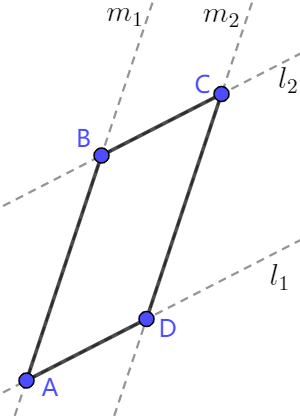
\includegraphics[width=0.3\textwidth]{tu/平行四边形0.png}
\end{wrapfigure}

设有四边形$ABCD$,我们说$AB$、$CD$互为\textbf{对边},$BC$、$DA$互为对边;
$\angle ABC$和$\angle CDA$互为\textbf{对角},$\angle BCD$和$\angle DAB$互为对角。
线段$AC$和$BD$称为四边形的\textbf{对角线}。

\begin{tm}\label{tm:0-0-0}
    平行四边形对边平行且等长,对角相等。
\end{tm}
\begin{proof}
    给定$\parasbx ABCD$,按定义可知对边平行。\\
    接着证明$\parasbx ABCD$的对角相等。\\
    $\angle ABC$和$\angle DAB$是同旁内角,所以和为平角。类似地,$\angle ABC$和$\angle BCD$是同旁内角,所以和为平角。于是,$\angle DAB = \angle BCD$。同理, $\angle ABC$和$\angle DAB$是同旁内角,所以和为平角。类似地,$\angle CDA$和$\angle DAB$是同旁内角,所以和为平角。于是,$\angle ABC = \angle CDA$。\\
    最后证明$\parasbx ABCD$的对边等长。\\
    连接对角线$AC$。$AB \parallel CD$,所以内错角$\angle CAB = \angle ACD$;同理,$BC \parallel DA$,所以内错角$\angle BCA = \angle DAC$。另外$|AC| = |AC|$。所以,根据“角边角”,$\triangle ABC \simeq \triangle CDA$。因此,$|AB| = |CD|$,$|BC| = |DA|$。    
\end{proof}

从证明中可以看出,平行四边形和三角形有密切的关系。把平行四边形沿对角线“裁开”,就得到一对同角全等的三角形。
一般来说,任何四边形沿对角线裁开,都会得到两个三角形。
因此,在约定角的范围是负平角到正平角时,\textbf{四边形的内角和是零角}。
对平行四边形来说,为了方便,也说它的内角和是周角。

除了对边分别平行,还有什么办法,判断一个四边形是不是平行四边形呢?
我们可以从这对全等三角形入手。以上证明中用到了“角边角”,是否可以换成“边角边”或“边边边”呢?

\begin{tm}\label{tm:0-0-1}
    对边等长的四边形是平行四边形。
\end{tm}
\begin{proof}
    设四边形$ABCD$中$|AB| = |CD|$,$|BC| = |DA|$。连接$AC$,根据“边边边”,
    $\triangle ABC \simeq \triangle CDA$,因此,$\angle CAB = \angle ACD$,
    于是$AB \parallel CD$。同理,由于$\angle BCA = \angle DAC$,$BC \parallel DA$。
    于是四边形$ABCD$是平行四边形。
\end{proof}

\begin{tm}\label{tm:0-0-2}
    一对边平行且等长的四边形是平行四边形。
\end{tm}
\begin{proof}
    设四边形$ABCD$中$AB \parallel CD$且$|AB| = |CD|$。连接$AC$。
    $|AC| = |AC|$。由于$AB \parallel CD$,内错角$\angle CAB = \angle ACD$。
    根据“边角边”,$\triangle ABC \simeq \triangle CDA$,因此,
    由于$\angle BCA = \angle DAC$,$BC \parallel DA$。于是四边形$ABCD$是平行四边形。
\end{proof}

\begin{tm}\label{tm:0-0-3}
    对角相等的四边形是平行四边形。
\end{tm}
\begin{proof}
    设四边形$ABCD$中$\angle ABC = \angle CDA$,$\angle BCD = \angle DAB$。
    四边形的内角和是两个平角,所以同旁内角$\angle ABC$和$\angle BCD$满足
    $\angle ABC + \angle BCD = 180^\circ$,这说明$AB \parallel CD$。
    同理,同旁内角$\angle ABC$和$\angle DAB$满足$\angle ABC + \angle DAB = 180^\circ$,
    因此$BC \parallel DA$。
\end{proof}

\begin{sk}\label{sk:0-0-0}
    一对边等长,一对角相等的四边形,是否是平行四边形?
\end{sk}

给定$\parasbx ABCD$,设对角线$AC$和$BD$的交点为$G$,我们把$G$叫做平行四边形的\textbf{中心}。
可以用“角边角”证明:$\triangle ABG \simeq \triangle CDG$,$\triangle BCG \simeq \triangle DAG$。
因此,$|AG| = |CG|$、$|BG| = |DG|$。$G$同时是两条对角线的中点。
换句话说,\textbf{平行四边形的两条对角线相互平分}。
用对称的说法,$A$和$C$关于$G$对称,$B$和$D$关于$G$对称。

在直角坐标系中,如果$A$的坐标是$(x_A, y_A)$,$B$的坐标是$(x_B, y_B)$,$C$的坐标是$(x_C, y_C)$,
$D$的坐标是$(x_D, y_D)$,那么$G$的坐标$(x_G, y_G)$满足:
$$ x_A + x_C = 2 x_G = x_B + x_D, \quad y_A + y_C = 2 y_G = y_B + y_D. $$

平行四边形还可以用来定义平移变换。直角坐标系中,我们已经定义过平移。
使用平行四边形的概念,设$A$是原点,那么关于另一点$B$的平移可以这样定义:
对平面上任一点$D$,作平行四边形$ABCD$,则$C$就是$D$平移后得到的点。
用坐标来表示的话,这个平移就是:
$$ (x_D, y_D) \mapsto (x_D + x_B, y_D + y_B).$$

\begin{xt}\label{xt:0-0-0}
    证明:\\
    1. 对角线相互平分的四边形是平行四边形。
\end{xt}

\section{特殊平行四边形}
平行四边形是对边平行、对角相等的四边形。下面我们来看几种特殊的平行四边形。

如果四边形四边等长,就说它是\textbf{菱形}。菱形肯定是平行四边形。
由于平行四边形对边等长,所以也可以这样判定菱形:
\begin{tm}\label{tm:0-1-0}
    邻边等长的平行四边形是菱形。
\end{tm}

\begin{wrapfigure}[9]{r}{0.25\textwidth} %this figure will be at the right
    \centering
    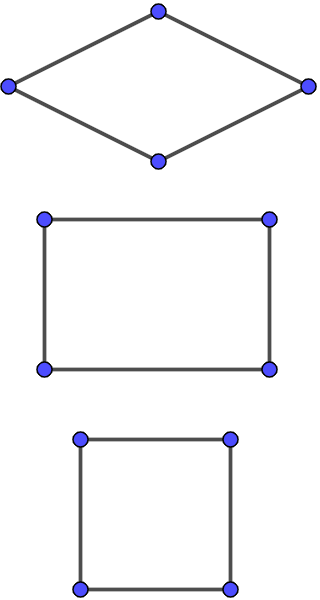
\includegraphics[width=0.24\textwidth]{tu/特殊平行四边形.png}
\end{wrapfigure}

把菱形沿对角线“裁开”,得到的一对三角形都是等腰三角形。
由于对角线平分,菱形的中心是等腰三角心底边中点,对角线也是中线。
而等腰三角形三线合一,中线就是高线。所以菱形的对角线不仅相互平分,而且相互垂直。

反过来,如果四边形的对角线相互平分,而且相互垂直,那么它是菱形。
菱形的两条对角线把它分为四个全等的直角三角形。

如果四边形四角相等,就说它是\textbf{矩形}或\textbf{长方形}。由于四边形内角和是周角,平行四边形对角相等,
所以也可以这样判定矩形:
\begin{tm}\label{tm:0-1-10}
    有一个角是直角的平行四边形是矩形。
\end{tm}

把矩形$ABCD$沿对角线$AC$“裁开”,得到$\triangle ABC$和$\triangle CDA$,
由于$\angle ABC$和$\angle CDA$都是直角,$\triangle ABC$和$\triangle CDA$是直角三角形。
根据勾股定理。$|AC|^2 = |AB|^2 + |BC|^2$。
另一方面,把矩形$ABCD$沿对角线$BD$“裁开”,通过类似推理可以得到:
$|BD|^2 = |AB|^2 + |AD|^2$。而$|BC| = |AD|$,所以$|AC| = |BD|$。即:
\begin{tm}\label{tm:0-1-15}
    矩形的对角线相互平分,而且等长。
\end{tm}

反过来,如果四边形的对角线相互平分而且等长,那么它是矩形。
矩形的两条把它分为两对全等的等腰三角形。

如果一个四边形既是菱形,又是矩形,就称它为\textbf{正方形}。
正方形是我们很熟悉的图形。正方形的四边等长,四个内角都是直角。
它的对角线长度是边长的$\sqrt{2}$倍。把正方形沿对角线“裁开”,得到一对等腰直角三角形。
正方形的两条对角线把它分为四个更小而全等的等腰直角三角形。

\section{梯形}
除了平行四边形,还有其他类型的四边形。

\begin{wrapfigure}[8]{r}{0.38\textwidth} %this figure will be at the right
    \vspace{-35pt}
    \centering
    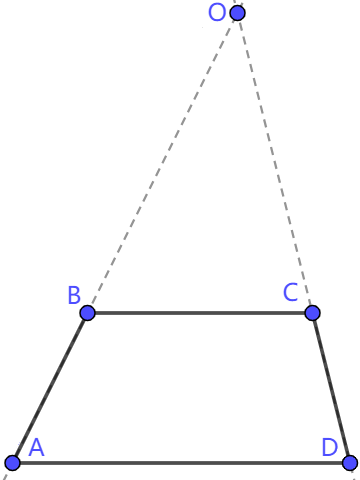
\includegraphics[width=0.36\textwidth]{tu/梯形1.png}
\end{wrapfigure}

如果四边形有一对边平行,就说它是\textbf{梯形}。如果梯形另一对边也平行,
就是平行四边形。我们已经研究过平行四边形了,所以,一般说梯形时,都指非平行四边形的梯形。

研究相似三角形的时候,我们已经接触过梯形。
如右图,大的三角形里去掉小的三角形,就是梯形。
把梯形补全为一对相似三角形,是常见的思考方式。

按照这个说法,梯形平行的一对边长度不等。我们称它们为\textbf{上底}和\textbf{下底}。
一般会把较短的一边称为上底,较长的称为下底。另外两条边一般称为梯形的\textbf{腰}。
两腰等长的梯形,称为\textbf{等腰梯形}。等腰梯形对应一对相似的等腰三角形。

设梯形$ABCD$中$BC \parallel AD$,那么同旁内角$\angle ABC + \angle DAB = 180^\circ$,
$\angle BCD + \angle CDA = 180^\circ$。如果其中一个角是直角,这样的梯形叫作\textbf{直角梯形}。
直角梯形对应一对相似的直角三角形。

梯形两腰的中点连线,称为梯形的\textbf{中位线}。
\begin{tm}\label{tm:0-2-20}
    梯形中位线长度是两底长度之和的一半。
\end{tm}
\begin{proof}
    设梯形$ABCD$中$BC \parallel AD$,$M$是边$AB$的中点,$N$是边$CD$的中点,
    直线$AB$、$CD$交于点$O$。由于$BC \parallel AD$,$\triangle OBC \sim \triangle OAD$。
    因此:
    $$ \frac{|OB|}{|OA|} = \frac{|OC|}{|OD|} = \frac{|BC|}{|AD|} = k.$$
    其中$k$是比例系数,即:
    $$ |OB| = k|OA|, \quad |OC| = k|OD|.$$
    于是
    $$ |OM| = |OB| + \frac{|AB|}{2} = \frac{|OA| + |OB|}{2} = \frac{k+1}{2} \cdot|OA|.$$
    同理,
    $$ |ON| = |OC| + \frac{|CD|}{2} = \frac{k+1}{2}\cdot|OD|. $$
    这说明
    $$ \frac{|OM|}{|OA|} = \frac{|ON|}{|OD|} = \frac{k+1}{2}. $$
    而$\angle MON = \angle AOD$,所以$\triangle OAD \sim \triangle OMN$。于是中位线$MN$的长度为
    $$ |MN| = |AD| \cdot \frac{|OM|}{|OA|} = \frac{k+1}{2}\cdot|AD|. $$
    将$k = \frac{|BC|}{|AD|}$代入,就得到
    $$ |MN| = \frac{|BC| + |AD|}{2}. $$
\end{proof}

\section{筝形}

\begin{wrapfigure}[6]{r}{0.32\textwidth} %this figure will be at the right
    \vspace{-5pt}
    \centering
    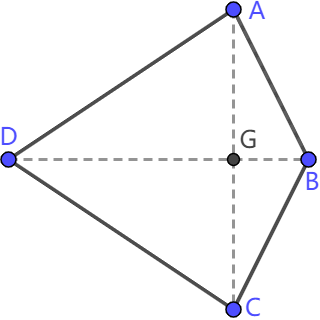
\includegraphics[width=0.32\textwidth]{tu/筝形1.png}
\end{wrapfigure}

平行四边形可以“裁成”两个同角全等的三角形。或者说,一对同角全等的三角形可以拼出一个平行四边形。
那么,一对反角全等的三角形拼出的图形是什么呢?

这个图形叫作\textbf{筝形}。我们对筝形并不陌生,在证明“角边角”的时候已经见过。
四边形的两对邻边分别等长,就叫作筝形。

如果筝形的对边也等长,就成了菱形。所以,一般说筝形时,都指非菱形的筝形。

筝形的最大特点,就是一条对角线是另一条的垂直平分线。我们把它叫作\textbf{脊线},
把另一条(被它平分的)对角线叫作\textbf{肩线}。我们已经证明过,脊线和肩线相互垂直。
它们把筝形分为两对全等直角三角形。

直角坐标系中,把$(0,0)$、$(0,a)$、$(a,a)$、$(a,0)$四点依次连起来,就围成一个边长为$a$的正方形。
如果把$(0,0)$、$(0,b)$、$(a,b)$、$(a,0)$四点依次连起来,就围成一个长宽为$a$和$b$的矩形。
如果把$(-a,0)$、$(0,b)$、$(a,0)$、$(0,-b)$四点依次连起来,就围成一个菱形。
如果把$(0,0)$、$(a,b)$、$(a+u,b+v)$、$(u,v)$四点依次连起来,就围成一个平行四边形。
这些形状可以看作是实心的点集。比如以上正方形对应点集:
$$\{(x,y) \,|\, 0\leqslant x, y \leqslant a\}.$$

从$(0,0)$、$(0,a)$、$(a,a)$、$(a,0)$连成的正方形出发,关于点$(0, a)$平移,
就得到一个新的正方形,它是$(0,a)$、$(0,2a)$、$(a,2a)$、$(a,a)$连成的正方形。

\begin{sk}\label{sk:5-3-0}
    \mbox{}\\
    \indent 1. 从一个(实心)正方形出发,通过平移,能否填满整个平面,不留空隙也不互相重叠?\\
    \indent 2. 从一个(实心的)矩形、菱形、平行四边形出发,通过平移,能否填满整个平面,不留空隙也不互相重叠?\\    
    \indent 3. 如果从一个(实心)图形出发,用和它全等的图形可以填满整个平面,不留空隙也不互相重叠,就说它是\textbf{密铺图形},可以密铺平面。
    正方形、矩形、菱形、平行四边形、等腰梯形、直角梯形、筝形,哪些是密铺图形?\\    
    \indent 4. 如果一个图形关于某条直线的轴对称图形是它自己,就说它是\textbf{轴对称图形},该直线是它的对称轴。
    同样,如果一个图形关于某点的中心对称图形是它自己,就说它是\textbf{中心对称图形},该点是它的对称中心。
    正方形、矩形、菱形、平行四边形、等腰梯形、直角梯形、筝形,哪些是轴对称图形,哪些是中心对称图形?
    它们分别有哪些对称轴和对称中心?
\end{sk}

\section{剪形和蝶形}
比较以下的四边形,它们相应的角度有什么不同?

% 平行四边形、剪形和蝶形
\begin{figure}[H] 
    \vspace{4pt}
    \centering
    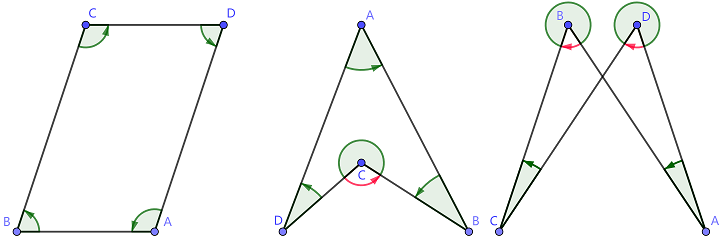
\includegraphics[width=0.8\textwidth]{tu/凹四边形1.png}
\end{figure}

给定四个点$A$、$B$、$C$、$D$,我们把线段$AB$、$BC$、$CD$、$DA$连起来的图形叫做四边形$ABCD$。
这四个顶点和四条边也组成了四个角:$\angle ABC$、$\angle BCD$、$\angle CDA$、$\angle DAB$。
我们称其为四边形$ABCD$的四个内角。

我们已经学习了平行四边形、梯形、筝形等四边形。如果把角的范围限定在\textbf{负平角}和\textbf{正平角}之间,
平行四边形的内角要么总是正的,要么总是负的。但也有一些四边形,它们的内角总是有正有负。
比如上图中间的四边形,内角$\angle BCD$是负的;上图右边的四边形,内角$\angle ABC$和$\angle CDA$是负的。

如果把这些四边形作轴对称,得到的四边形内角恰好与原本相反。上图中间的四边形会变成有三个内角为负的四边形;
右边的四边形仍旧是两个内角为负的四边形。

我们把类似上图中间的四边形,内角中有一个或三个为负的,称为\textbf{剪形};
把类似上图右边的四边形,内角中有两个为负的,称为\textbf{蝶形}。

蝶形和剪形合称为\textbf{凹四边形},其余内角总为正或总为负的四边形,称为\textbf{凸四边形}。
平行四边形总是凸四边形。梯形也可以是蝶形,筝形也可以是剪形。

\begin{sk}\label{sk:5-4-0}
    \mbox{}\\
    \indent 1. 梯形在什么情况下是蝶形?画一个例子。\\
    \indent 2. 筝形在什么情况下是剪形?画一个例子。\\
    \indent 3. 考虑四边形内角的正负。凸四边形的内角是“正-正-正-正”或“负-负-负-负”;
    剪形的内角是“正-正-正-负”或“正-负-负-负”;蝶形的内角是“正-正-负-负”。是否有其他的可能组合?
    哪些正负组合是不可能的?为什么?
\end{sk}

\section{四边形的面积}
学习了各种常见的基本图形后,最后来看它们的面积。我们已经学习过正方形、矩形、平行四边形和三角形的面积公式。
现在,我们把这些性质归纳成公理。

\begin{wrapfigure}[4]{r}{0.36\textwidth} 
    \vspace{-30pt}
    \flushright
    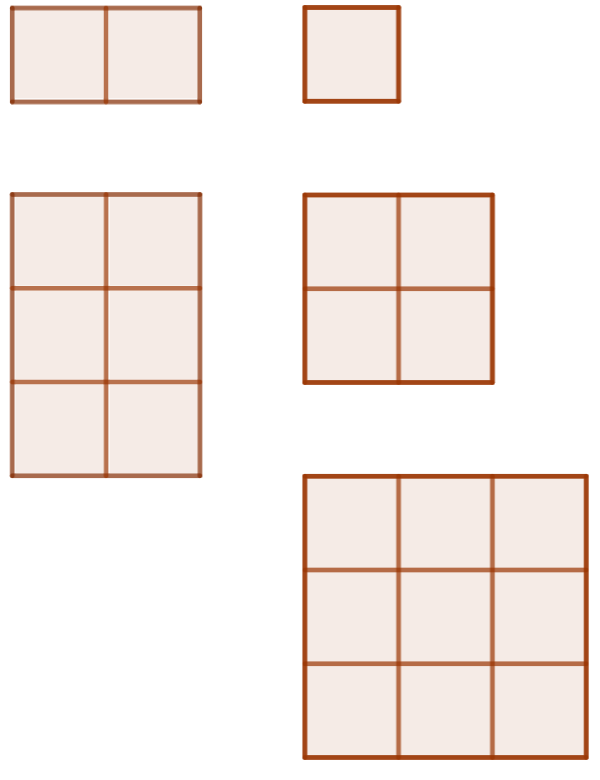
\includegraphics[width=0.32\textwidth]{tu/面积_矩形1.png}
\end{wrapfigure}

我们把正方形作为面积的单位。
\begin{po}
    边长为一的正方形,面积为一。
\end{po}

我们把边长为一的正方形称为\textbf{单位正方形}。怎样从单位正方形得到其他图形的面积呢?

回顾(右图):我们是怎样数出正方形乃至矩形面积的。

\begin{po}
    图形的面积是其各部分面积之和。
\end{po}

\begin{po}
    图形平移、旋转后,面积不变。对称的图形,面积相等。
\end{po}
这两个公理给出了从单位正方形得到其他图形的面积的方法。
从单位正方形出发,我们可以得到矩形、平行四边形、三角形的面积公式。

\begin{figure}[H] %this figure will be at the right
    \vspace{4pt}
    \centering
    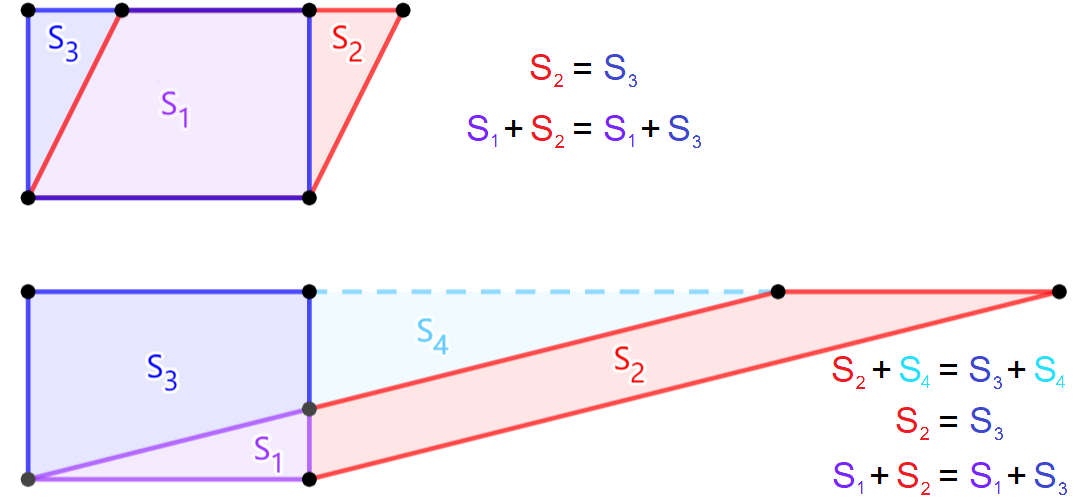
\includegraphics[width=0.6\textwidth]{tu/面积_平行四边形1.png}
\end{figure}

\begin{itemize}
    \item 正方形的面积等于边长的平方。
    \item 矩形的面积等于长乘宽。
    \item 平行四边形的面积等于同底等高的矩形的面积,即底乘高。
    \item 三角形的面积是同底等高平行四边形的一半,即底乘高的一半。
\end{itemize}

同底等高的平行四边形的面积,都等于和它们同底等高的矩形的面积。
同底等高的三角形的面积,分别为同底等高的平行四边形的面积的一半。因此我们得出熟知的结论:
\begin{tm}
    同底等高的平行四边形面积相等。同底等高的三角形面积相等。
\end{tm}

梯形的面积,可以通过将两个梯形拼成一个平行四边形而求得。
筝形的面积,可以通过将对角线分成的四个三角形旋转,拼成矩形而求得。

\begin{figure}[H] 
    \vspace{4pt}
    \centering
    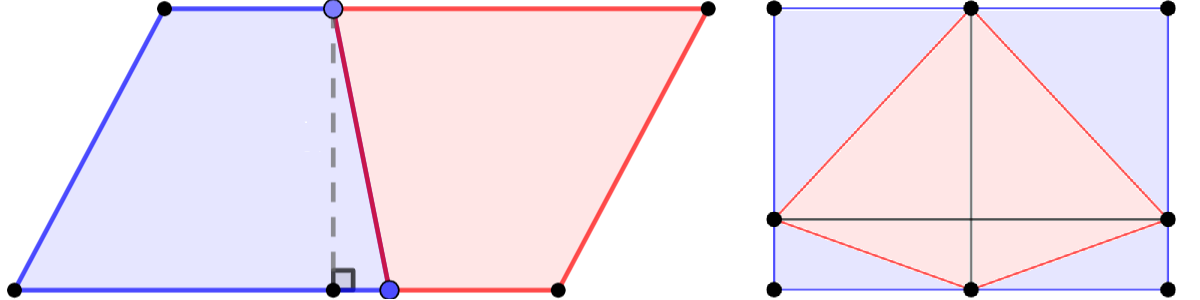
\includegraphics[width=0.8\textwidth]{tu/面积_梯形1.png}
\end{figure}

\begin{itemize}
    \item 梯形的面积等于上下底边长之和乘高除以2。
    \item 筝形的面积等于对角线乘积的一半。
\end{itemize}

怎样求一般的四边形,乃至多边形的面积呢?讨论四边形内角和的时候,我们已经发现,
可以沿着对角线把任何多边形划分成若干个三角形。因此,四边形乃至多边形的面积,就是这些三角形面积之和。
也就是说,只要能够求出任意形状三角形的面积,就能求出任意四边形乃至多边形的面积。
这个问题我们将会在后续章节中讨论。

多边形是由线段首尾相接连成的。
如果平面图形的边不是线段,如何讨论它们的面积呢?

观察下图,图形完整覆盖了多少个方格?有多少个方格覆盖了图形?你有什么想法?

\begin{figure}[H] 
    \vspace{4pt}
    \centering
    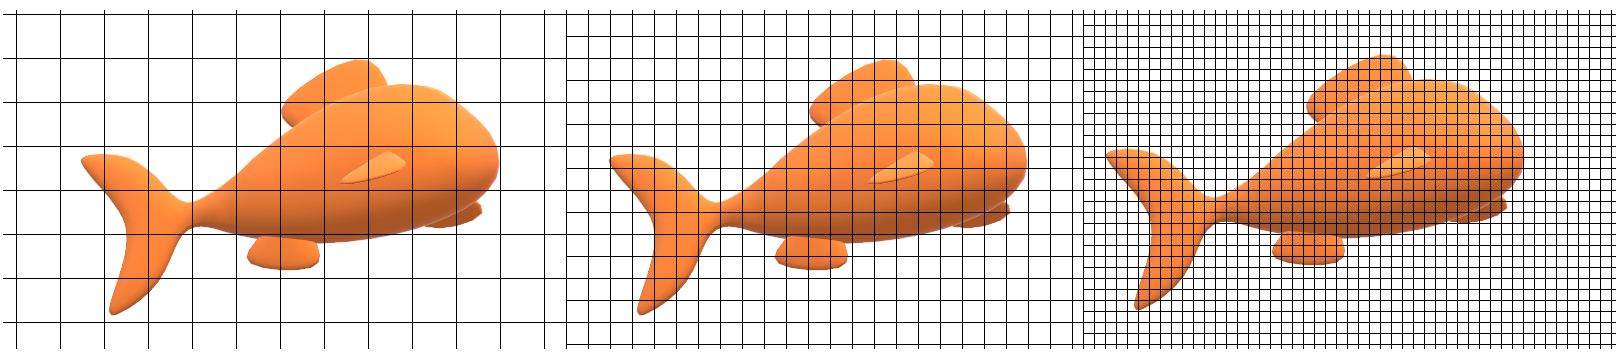
\includegraphics[width=0.8\textwidth]{tu/面积_鱼1.png}
\end{figure}

上图中,我们把一张透明方格网纸放在图形上。图形的面积$S$大于等于它完整覆盖的方格数$N_{\text{内}}$,
同时小于等于把它完整覆盖所用的方格数$N_{\text{外}}$。设每个方格面积为$S_1$,
那么$S$介于$N_{\text{内}}S_1$和$N_{\text{外}}S_1$之间。如果随着方格面积缩小,
$N_{\text{内}}S_1$和$N_{\text{外}}S_1$的差也逐渐缩小,那么我们就能越来越精确地估计图形的面积。

\begin{sk}
    \mbox{} \\
    \indent 1. 是否所有平面图形都有面积?怎样界定一个图形是否有面积?
\end{sk}

\begin{xt}
    \mbox{} \\

    \begin{figure}[H] 
        \vspace{4pt}
        \centering
        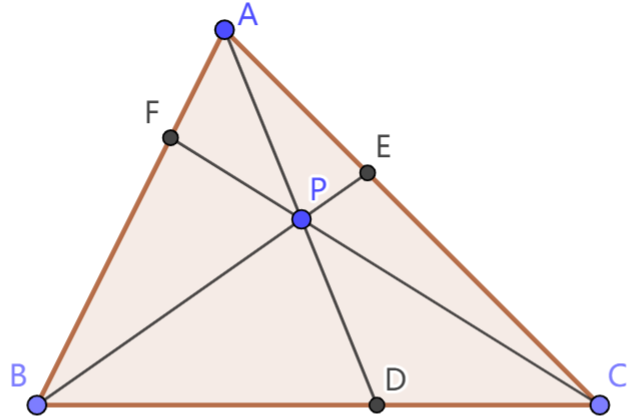
\includegraphics[width=0.45\textwidth]{tu/塞瓦定理1.png}
    \end{figure}

    \indent 1. 给定三角形$ABC$及其内一点$P$,从三角形各个顶点出发的射线$AP$、$BP$、$CP$
    分别交对边$BC$、$AC$、$AB$于$D$、$E$、$F$。\\
    \indent 1.1 证明:
    $$ \frac{|AF|}{|FB|} = \frac{S_{\triangle ACF}}{S_{\triangle FCB}}\,\,.$$
    \indent 其中$S_{\triangle ACF}$表示三角形$ACF$的面积。余皆同。\\
    \indent 1.2 证明:
    $$ \frac{|AF|}{|FB|} = \frac{S_{\triangle ACP}}{S_{\triangle PCB}}\,\,.$$
    \indent 1.3 证明:
    $$ \frac{|AF|}{|FB|} \cdot \frac{|BD|}{|DC|} \cdot \frac{|CE|}{|EA|} = 1\,\,.$$
    \indent 1.4 证明:
    $$ \frac{|AP|}{|PD|} = \frac{S_{\triangle ACP}}{S_{\triangle PCD}}\,\,.$$
    \indent 1.5 证明:
    $$ \frac{|AP|}{|PD|} \cdot \frac{|DC|}{|CB|} \cdot \frac{|BF|}{|FA|} = 1\,\,.$$
    \indent 1.6 你还能发现哪些类似的等式?
\end{xt}


\chapter{数的分解}
自然数是我们最早认识的数。我们已经熟悉了自然数的四则运算,并且学习了因数和倍数。
了解一个数的因数,无论对于理论研究,还是在实际生活中,都很有用处。
\section{初识素数}
我们已经学习过因数的概念。我们把因数只有自己和$1$的正整数叫做\textbf{素数},
除了$1$和自己还有别的因数的正整数叫做\textbf{合数}。约定$1$既不是素数也不是合数。

举例来说,$2$、$3$、$5$、$7$是素数,而$4$、$6$、$8$是合数。偶素数只有一个:$2$,其余素数都是奇数。

\begin{tm}\label{tm:1-0-0}
    设$p$是素数。任何正整数要么是$p$的倍数,要么与$p$互素。
\end{tm}
\begin{proof}
    设$n$是正整数。记$n$和$p$的最大公因数为$d$。$d$是$p$的因数。
    因此按$p$的定义,要么$d = p$,要么$d = 1$。
    如果$d = p$,那么$n$是$p$的倍数。如果$d = 1$,那么$n$与$p$互素。
\end{proof}

素数与合数有什么关系呢?

\begin{tm}\label{tm:1-0-4}
    合数总有素因数。
\end{tm}
\begin{proof}
    按照定义,合数总有真因数。给定合数$n$,它的真因数大于$1$、小于$n$,至少有一个,至多有$n-2$个。
    其中总有一个最小的真因数,我们把它记为$p$。\\
    $p$的因数也是$n$的因数,所以要么是$1$,要么大于等于$p$。也就是说,$p$没有真因数。所以$p$是素数。
\end{proof}

\begin{tm}\label{tm:1-0-6}
    每个大于$1$的整数都可以表示成素数或其乘积。
\end{tm}
\begin{proof}
    使用归纳法。命题$P(n)$:整数$n$可以表示成素数或其乘积。下面证明$P$对每个大于$1$的整数成立。\\
    $n=2$时,由于$2 = 2$,$P(2)$成立。\\
    假设对某个大于$1$的整数$n$,$P(2), \cdots, P(n)$都成立,下面证明$P(n+1)$也成立。\\
    如果$n+1$是素数,那么$n+1 = n+1$就是素数,于是$P(n+1)$成立。\\
    如果$n+1$是合数,那么它至少有一个素因数$p$。设$n+1 = mp, m\in\mathbb{Z}^+$,
    由于$1<p<n+1$,所以$1< m < n+1$。根据假设,$P(m)$成立,也就是说,
    $m$可以表示成素数或其乘积:
    $$ m = p_1 p_2\cdots p_k, \,\,\, l\in\mathbb{Z}^+$$
    于是,$n+1 = mp = pp_1 p_2\cdots p_k$也是素数的乘积。于是$P(n+1)$成立。\\
    综上所述,$P(n)$对每个大于$1$的整数成立。
\end{proof}

我们把这种表示正整数的方式称为\textbf{素因数分解}。
如果把自然数比作一座座房屋,那么素数就是砖瓦,构建起一个个合数。

素数与合数,谁比较多呢?一位数中,有$4$个素数,$4$个合数;二位数中,有$21$个素数,$69$个合数;
三位数中,有$143$个素数,$757$个合数;四位数中有$1061$个素数,$7939$个合数。

越大的素数,越是罕见。

会不会从某个数开始,所有比它大的都是合数?也许,素数只有有限个?我们有这样一个定理:

\begin{tm}\label{tm:1-0-10}
    素数的个数是无穷的。
\end{tm}
\begin{proof}
    使用反证法证明。反设素数的个数不是无穷的,即只有有限多个素数。把素数的个数记为$N$,把它们从小到大分别记为
    $p_1, p_2,\cdots , p_N$。\\
    考察这样的正整数:
    $$ m = p_1p_2\cdots p_N + 1.$$
    $m$与所有素数互素。所以,$m$的因数要么是$1$,要么是它自己,要么是某个与$p_1$、$p_2$、……、$p_N$都不一样的数。
    这就说明,要么$m$自己是素数,要么它的因数中有和$p_1, p_2,\cdots , p_N$都不一样的素数。
    这就和“素数一共有$N$个”矛盾了。\\
    因此,原命题的否定“素数的个数不是无穷的”是假的,原命题成立。
\end{proof}

素数作为“砖瓦”的性质,还体现在以下定理中:
\begin{tm}{\textbf{存因定理 }}\label{tm:1-0-20}
    如果素数$p$整除两个自然数$a$和$b$的乘积:$p | ab$,那么$p$整除$a$或$p$整除$b$。
\end{tm}
\begin{proof}
    给定符合条件的素数$p$和自然数$a,b$。如果$p$整除$a$,那么命题得证。\\
    如果$p$不整除$a$,那么由于两者的最大公因数是$p$的因数,因此只能是$1$。两者互素。
    根据倍和析因定理,存在整数$m,n$使得
    $$ mp + na = 1.$$
    两边乘以$b$,就得到:
    $$ mp + nab = b. $$
    根据已知条件,存在整数$k$使得$ab = kp$,于是 
    $$ b = mp + nkp = (m + nk)p,$$
    即$p$整除$b$。
\end{proof}

存因定理告诉我们,如果某个正整数$n$有素因数$p$,把$n$“拆成”两个数的乘积,那么总有一个有素因数$p$。
反复运用存因定理,我们可以把这个结论加强:无论把$n$“拆成”几个数的乘积,总有一个有素因数$p$。
这反映了素数作为自然数中的“砖瓦”的性质。

\begin{xt}\label{xt:1-0-0}
    证明:\\
    \indent 1. 两个素数要么相等,要么互素。\\
    \indent 2. 如果素数$p$整除完全平方数$n$,那么$p^2$也整除$n$。\\
    \indent 3. 设$p,q$是素数,$i,j$是正整数,那么要么$p^i$和$q^j$互素,要么$p^i$整除$q^j$,要么$q^j$整除$p^i$。\\
    \indent 4. 对任何正整数$n$,都存在$n$个连续合数$a, a+1, \cdots , a+n-1$。
\end{xt}

\section{算数基本定理}
从存因定理出发,可以得到一个很重要的结论:
\begin{tm}{\textbf{算术基本定理}}\label{tm:1-1-0}
    如果不考虑素因数的排列顺序,素因数分解的方式是唯一的。
\end{tm}
\begin{proof}
    如果某个大于$1$的整数$n$有两种素因数分解。把每种分解的素因数从小到大排列:
    $$ n = p_1p_2\cdots p_k = q_1q_2\cdots q_l, \,\,\, k, l \in \mathbb{Z}^+.$$
    我们要证明这两种分解是一样的。\\
    考虑$p_1$,$p_1$整除$n = q_1q_2\cdots q_l$。根据存因定理,存在某个$j$使得$p_1$整除$q_j$。
    $q_j$也是素数,所以$p_1$不可能是它的真因数。于是$p_1 = q_j \geqslant q_1$。\\
    考虑$q_1$,按照相同的推理,存在某个$i$使得$q_1$整除$p_i$。于是$q_1 = p_i \geqslant p_1$。\\
    因此,$p_1 = q_1$。\\
    我们把$n$除以$p_1$,得到正整数$n_1$。如果$n_1 = 1$,那么我们有$n_1 = p_1$,分解方式是唯一的。
    如果$n_1 = p_2\cdots p_k = q_2\cdots q_l > 1$,我们可以再次运用以上的推理,得到:$p_2 = q_2$。\\
    以此类推,经过有限步后,我们可以得到:$k=l$,且
    $$p_1 = q_1, \,\,\, p_2 = q_2, \, \cdots \, , p_k = q_k.$$
    也就是说,$n$的素因数分解只有一种方式。
\end{proof}

这个结论非常重要,我们把它称为算术基本定理。算术基本定理告诉我们,不考虑排列顺序的话,
每个大于$1$的正整数都可以用唯一的方式写成素数或其乘积。这种唯一的方式可以看作每个正整数的
“身份证”。为了方便讨论,素因数分解中,一般素因数从小到大排列,并用乘方的形式合并相同的素因数。
比如,$252$的素因数分解写成;
$$ 252 = 2^2 \cdot 3^2 \cdot 7^1.$$
这种写法称为数的\textbf{标准分解}。以上就是$252$的标准分解。
有时候,为了便于讨论,我们会把不是$n$的因数的素数也写进分解表达式里,用它的$0$次方“占位”.比如$210$
就可以写成:
$$ 252 = 2^2 \cdot 3^2 \cdot 5^0 \cdot 7^1.$$
这样的写法,在规定了涉及的素数集合后,仍然是唯一的。

\begin{xt}\label{xt:1-1-0}
    写出以下数的标准分解:\\
    \indent 1. $256, 243, 125$.\\
    \indent 2. $60, 780, 1296$.\\
    \indent 3. $1001, 5929, 8801$.
\end{xt}

把正整数$n$分解,得到:$n = p_1^{u_1} p_2^{u_2} \cdots p_k^{u_k}$。
我们把$u_1$称为$p_1$在$n$中的重数。它是让$p_1^i$整除$n$的最大自然数$i$。
\begin{tm}\label{tm:1-1-10}
    如果$n$整除$m$,那么任何素数在$n$中的重数小于等于它在$m$中的重数。
\end{tm}
\begin{proof}
    设素数$p$在$n$和$m$中的重数分别是$u$和$v$。于是$p^u$整除$n$,因而整除$m$。
    另一方面,$v$是让$p^i$整除$m$的最大自然数$i$。所以,$u \leqslant v$。
\end{proof}

上面的结论也可以换个方式说成:如果$n$是$m$的因数,那么任何素数在$n$中的重数小于等于它在$m$中的重数;
如果$n$是$m$的倍数,那么任何素数在$n$中的重数大于等于它在$m$中的重数。

\begin{tm}\label{tm:1-1-20}
    正整数$n,m$的乘积,等于它们的最大公因数和最小公倍数的乘积。
\end{tm}
\begin{proof}
    设$n,m$的最大公因数是$d$,最小公倍数是$q$,下面证明$nm = dq$。\\
    把$n,m,d,q$分解,设涉及的素数为$p_1, p_2, \cdots , p_k$。把四个数分别记为:
    \begin{align*}
        n &= p_1^{u_1}p_2^{u_2}\cdots p_k^{u_k}, \quad m = p_1^{v_1}p_2^{v_2}\cdots p_k^{v_k},  \\
        d &= p_1^{s_1}p_2^{s_2}\cdots p_k^{s_k}, \quad q = p_1^{t_1}p_2^{t_2}\cdots p_k^{t_k}.  
    \end{align*}
    $d$既是$n$的因数也是$m$的因数,所以对每个素因数$p_i$,它在$d$中的重数$s_i$都小于等于$u_i$和$v_i$。
    同时,由于$d$是最大公因数,所以$s_i$是$u_i$和$v_i$中较小的数。\\
    $q$既是$n$的倍数也是$m$的倍数,所以对每个素因数$p_i$,它在$q$中的重数$t_i$都大于等于$u_i$和$v_i$。
    同时,由于$q$是最小公倍数,所以$t_i$是$u_i$和$v_i$中较大的数。\\
    因此,对每个素因数$p_i$,$s_i + t_i = u_i + v_i$。于是,
    \begin{align*}
        nm &= \left(p_1^{u_1}p_2^{u_2}\cdots p_k^{u_k}\right) \cdot \left(p_1^{v_1}p_2^{v_2}\cdots p_k^{v_k}\right)  \\
        &= p_1^{u_1 + v_1}p_2^{u_2 + v_2}\cdots p_k^{u_k + v_k}  \\
        &= p_1^{s_1 + t_1}p_2^{s_2 + t_2}\cdots p_k^{s_k + t_k}  \\
        &= \left(p_1^{s_1}p_2^{s_2}\cdots p_k^{s_k}\right) \cdot \left(p_1^{t_1}p_2^{t_2}\cdots p_k^{t_k}\right)  \\
        &= dq 
    \end{align*}    

\end{proof}

\begin{xt}\label{xt:1-1-1}
    \mbox{}\\
    \indent 1. 设$i$是素数$p$在正整数$n$中的重数。\\
    \indent 1. 1. 如果$p$不整除$n$,证明$i = 0$。\\
    \indent 1. 2. 如果自然数$j < i$,证明:$p^j$整除$n$。\\
    \indent 1. 3. 如果自然数$j > i$,证明:$p^j$不整除$n$。\\
    \indent 2. 设正整数$n,m$的最大公因数是$d$,素数$p$在$d,n,m$中的重数分别是$s,u,v$。\\
    \indent 2. 1. 设$v$是$u,v$中较小的数,证明:$s \leqslant v$。\\
    \indent 2. 2. 假设$s < v$,考虑$pd$,证明$pd$是$n,m$的公因数。\\
    \indent 2. 3. 证明$s$等于$u,v$中较小的数。 \\
    \indent 2. 4. 设正整数$n,m$的最小公倍数是$q$,素数$p$在$q,n,m$中的重数分别是$t,u,v$,证明:$t$等于$u,v$中较大的数。\\
\end{xt}

给定一个正整数,如何将它分解呢?这个问题一直困扰着人类。将非常大的整数分解,是一项非常困难的任务。
即便在现代,电子计算机计算能力有极大发展,可以轻易做到每秒百亿乃至万亿次运算,分解大整数仍然需要非常多的时间。
一些常用的密码技术,就依赖于分解大整数非常困难这个事实。

如今,量子计算理论不断发展。人们将希望寄于量子计算机,认为将来使用量子计算机及相应的算法,
可以在合理时间内分解大整数。

\chapter{因式分解}
整式是变量和数量作加减法和乘法得到的代数式。它的性质和整数很相似。
整数可以分解成因数的乘积,整式也可以分解为整式的乘积。
把整式的乘积写成若干项的和,叫做整式的展开;
反过来,把一个整式写成多个整式的乘积,称为整式的\textbf{因式分解}。乘积中每个整式称为原整式的\textbf{因式}。

整式的因式分解是一个非常庞大的问题。我们只从最简单的情况出发,归纳一些特殊情况下的简单方法。

\section{一元整式}
一种简单的情况是一元整式的因式分解。给定变量为$x$的一元整式$p$,合并同类项后按照次数从高到低排列,可以写成:
$$ p = a_nx^n + a_{n-1}x^{n-1} + \cdots + a_1 x + a_0.$$
其中$a_0, a_1, \cdot , a_n$都是有理数,称为$p$的系数。其中$a_n$不等于$0$,而其它数可能等于$0$。
$a_nx^n$称为$p$的\textbf{最高次项},$a_n$就是最高次项的系数,$n$称为$p$的次数。比如$n=1$时,$p$
就是我们见过的一元一次式。$n=0$时,$p$只有常数项,称为常式。为了强调$p$是关于$x$的一元式,我们也将$p$记为$p(x)$。

给定一元整式$n(x)$和$m(x)$,如果$n(x)$可以写成$m(x)$和另一个一元整式$q(x)$的乘积,
就说$n(x)$是$m(x)$的\textbf{倍式},$m(x)$是$n(x)$的\textbf{因式}。

和整数一样,一元整式也有带余除法。整式的带余除法可以和整数除法一样,用竖式计算。
比如$8x^5 +2x^4 -9x^3+ 4x-5$除以$2x^2+x-1$:
$$\polylongdiv{8x^5 +2x^4 -9x^3+ 4x-5}{2x^2+x-1}$$
可以看到,\textbf{被除式}$8x^5 +2x^4 -9x^3+ 4x-5$除以\textbf{除式}$2x^2+x-1$,得到\textbf{商式}$4x^3-x^2-2x+\frac12$和\textbf{余式}$\frac32 x- \frac92$。
竖式除法中,不同次数的项就好像整数的个十百千等数位。不同的是相减的时候没有借位,而且由于系数可以是分数,
所以只要剩下的式子的次数不少于除式,就可以继续相减。最后得到的余式,次数一定严格小于除式。
\begin{sk}\label{sk:2-0-0}
    整式$p(x)$除以一次式,余式是怎样的?除以常式呢?
\end{sk}
\begin{xt}\label{xt:2-0-0}
    计算带余除法:\\
    1. $x^3 - 3x^2 + 2x - 5$除以$x^2 + x + 2$。\\
    2. $x^6 - x^5 - 4x^3 + 11x^2 - 9x + 19$除以$x^3 - 2x^2 + x + 4$。
\end{xt}

\section{试根法}
怎么样找到一元整式的因式呢?我们来看上面的整式除法。

当$x=1$的时候,$2x^2+x-1 = 2$,$8x^5 +2x^4 -9x^3+ 4x-5 = 0$,
$4x^3-x^2-2x+\frac12 = \frac32$,$\frac32 x- \frac92 = -3$。
带余除法变成:$0 = 2 \cdot \frac32 - 3$。

用特定的数值代替$x$,整式的带余除法就变成整数的带余除法。如果$x$取某个值使得除式$2x^2 + x - 1 = 0$,
比如$x = -1$,那么带余除法变成:$-6 = 0\cdot \left(\frac52\right) - 6$。

如果$2x^2 + x - 1$是某个一元整式$p(x)$的因式,
$$ p(x) = (2x^2 + x - 1)q(x)$$
那么,某个$x$的取值(比如$-1$)使得$2x^2 + x - 1 = 0$的时候,上式变成:
$$ p(-1) = 0 \cdot q(-1) = 0$$
如果某个数$a$使整式的因式等于$0$,那么它也使得整式为$0$。

使整式为$0$的数叫做整式的\textbf{根}。

如果某个数$a$使除式为$0$,被除式也为$0$,除式是否就是被除式的因式呢?
考虑带余除法:
$$\polylongdiv{8x^5 +2x^4 -9x^3+ 4x+1}{2x^2+x-1}$$
$x = -1$的时候,除式和被除式都是$0$,但这是由于$x = -1$时余式也是$0$。
除式并不是被除式的因式。

不过,如果余式是常式,那么它是不是$0$,就和$x$的取值无关了。
一种特殊情况是:除式是一次式:$x - a$。它只在$x$取值为$a$的时候为$0$。
这时,如果被除式也是$0$,那么余式肯定是$0$。于是除式是被除式的因式。
\begin{tm}\textbf{余式定理}\label{tm:2-1-0}
    \mbox{} \\
    如果$a$是一元整式$p(x)$的根,那么$x-a$是它的因式。
\end{tm}

\begin{xt}\label{xt:2-1-0}
    \mbox{}\\
    设有整式$p = 6x^3 - 3x^2 + 2x - 1$:\\
    \indent 1. 试着分解$p$。\\
    \indent 2. 如果既约分数$\frac{a}{b}$是$p$的根,证明:$|b|$整除$6$。\\
    设有整式$p = x^3 - 4x^2 - x - 20 $:\\
    \indent 1. 试着分解$p$。\\
    \indent 2. 如果既约分数$\frac{a}{b}$是$p$的根,证明:$|a|$整除$20$。\\
    如果既约分数$\frac{a}{b}$是整式$p = a_nx^n + a_{n-1}x^{n-1} + \cdots + a_1 x + a_0$的根,
    $a$和$b$应该满足什么条件?
\end{xt}

\section{一般整式的分解}
对一般的整式来说,也有一些普遍适用的方法。

\noindent \textbf{提公因式法}

\indent 如果要分解的整式中有显然的公因式,那么可以将它提取出来。比如:
$$ x^6 - 2x^4 + 19 x^3 -3x$$
\indent 以上这个式子中,每一项显然都有$x$作为因式。因此,可以分解为:
$$ x(x^5 - 2x^3 + 19x^2 - 3).$$
\indent 提公因式法是分配律的逆应用。

\noindent \textbf{公式法}

\indent 如果可以注意到要分解的整式是某个公式的展开形式,那么应用公式,
\indent 就可以把展开的形式还原成因式的成绩形式。比如: 
$$x^4 + 4$$
\indent 这个式子可以看成两个平方的差:
$$ x^4 + 4 = x^4 - 4x^2 + 4 - 4x^2 = (x^2 - 2)^2- (2x)^2.$$
\indent 于是,使用$a^2 - b^2 = (a + b)(a - b)$这个公式,就可以得到:
$$x^4 + 4 = (x^2 - 2 + 2x)(x^2 -2 -2x).$$
\indent 应用公式法,取决于要分解的整式是否符合某个特定公式的展开形式。

\noindent \textbf{分组分解法}

\indent 分组分解的思想是从提公因式法出发。如果不能发现显然的公因式,
\indent 就分组考察整式的项,看看是不是有哪些项可以先提取公因式。比如:
$$ ab + abc - a^2 - b^2c$$
\indent 可以先把上式的项分为两组:
$$ ab + abc - a^2 - b^2c = (ab - a^2) + (abc - b^2c)$$
\indent 然后分别对每一组做因式分解:
$$ ab + abc - a^2 - b^2c = (ab - a^2) + (abc - b^2c) = a(b - a) + bc(a - b)$$
\indent 然后再提取公因式$a - b$:
$$ ab + abc - a^2 - b^2c = a(b - a) + bc(a - b) = (a - b)(-a + bc).$$
\indent 可以看到,分组分解的关键在于:各组各自分解的结果,应该有共同的\\
\indent 因式。比如上式分成两组,每组都分解出了$a - b$这个因式。

\noindent \textbf{待定系数法}

\indent 如果对因式分解的结果有一定的猜测,可以先用变量代替暂时不知道\\
\indent 的系数,写出因式乘积。展开后,通过对比各项,得到系数。比如:
$$ 3ab + ac - a^2- bc -2b^2 $$
\indent 上式中,让$a = b$,则式子变为:
$$ 3ab + ac - a^2- bc -2b^2 = 3b^2 + bc - b^2- bc -2b^2 = 0$$
\indent 所以,猜测$a - b$是因式。由于式子最高次项次数是$2$,猜测因式分解\\
\indent 结果为:
$$ 3ab + ac - a^2- bc -2b^2 = (a - b)(ua + vb + wc).$$
\indent 展开后得到:
$$ 3ab + ac - a^2- bc -2b^2 = ua^2 + vb^2 + (v - u)ab + wac - wbc. $$
\indent 对比左右各项,得到$u = -1$、$v = 2$、$w = 1$。即:
$$ 3ab + ac - a^2- bc -2b^2 = (a - b)(-a + 2b + c).$$
\indent 待定系数法建立在对因式分解结果的合理猜测上。如果猜测出现错误,
\indent 后面对比各项时就会发现矛盾。


\chapter{二次方根和二次根式}
分式开平方得到的代数式,叫做\textbf{二次根式}。二次根式可以看成用代数式代替二次方根$\sqrt{q}$中的数量$q$得到的结果。
$\sqrt{c}$、$\sqrt{1 - a + a^2}$、$\sqrt{x^3 - x^2 - 2}$等都是二次根式。通过二次根式,我们可以更好地理解二次方根的性质。
\section{二次方根的化简}
\begin{sk}\label{sk:3-0-0}
    以下二次方根有什么联系?\\
    \indent 1. $\sqrt{2}$、$\sqrt{8}$、$\sqrt{72}$.\\
    \indent 2. $\sqrt{3}$、$\sqrt{45}$、$\sqrt{147}$.\\
    \indent 3. $\sqrt{5}$、$\sqrt{\frac{5}{4}}$、$\sqrt{\frac{20}{49}}$.
\end{sk}
如果正整数$n$有完全平方数$a^2$作为因数\footnote{其中$a>1$,下同。}:$n = ma^2$,那么
$$\sqrt{n} = \sqrt{m}\sqrt{a^2} = a\sqrt{m}.$$
用这个方法,可以把正整数$n$的二次方根$\sqrt{n}$写成一个整数$a$和一个无理数$\sqrt{m}$的乘积。其中$m$没有完全平方数作为因数,
所以$\sqrt{m}$是无理数。我们把这样的形式称为$\sqrt{n}$的\textbf{最简形式},把找到最简形式的过程称为
(整数)二次方根的化简。

要化简整数的二次方根,可以先把整数分解成素因数的乘积。给定(大于$1$的)正整数$n$,写出它的标准分解:
$$n = p_1^{u_1} p_2^{u_2} \cdots p_k^{u_k}$$
如果某个素因数$p_i$在$n$中的指数$u_i$是偶数,那么$p_i^{u_i}$是一个完全平方数;
如果$u_i$是奇数,那么$p_i^{u_i-1}$是一个完全平方数。于是,我们可以把$n$的素因数分为两类,
一类是指数为偶数的,另一类是指数为奇数的。我们可以把前一类中的$p_i^{u_i}$和后一类的$p_i^{u_i-1}$提出来,
相乘得到一个完全平方数。剩下的就是指数为奇数的素因数的乘积。如果我们定义这样的函数:
$$ \varsigma: n = p_1^{u_1} p_2^{u_2} \cdots p_k^{u_k} \mapsto p_1^{r_1} p_2^{r_2} \cdots p_k^{r_k}. $$
其中的$r_1, r_2, \cdots r_k$分别是$u_1, u_2, \cdots u_k$除以$2$的余数。那么$\varsigma(n)$就是剩下的指数为奇数的素因数的乘积。
而$\frac{n}{\varsigma(n)}$是一个完全平方数。

$\varsigma(n)$已经没有完全平方数的因子了,我们把它叫做$n$的\textbf{二次方余}。$n$可以写成:
$$ \sqrt{n} = a\sqrt{\varsigma(n)}.$$
其中正整数$a$是$\frac{n}{\varsigma(n)}$的平方根。

举例来说,要化简$\sqrt{2520}$,可以先把正整数$2520$分解:
$$ 2520 = 2^3 \cdot 3^2 \cdot 5 \cdot 7.$$
然后提出完全平方的部分,计算方余:
$$ 2520 = \left(2^2 \cdot 3^2 \right) \cdot (2 \cdot 5 \cdot 7)$$
因此$\varsigma(n) = 2 \cdot 5 \cdot 7 = 70$,
$$ \sqrt{2520} = 6 \sqrt{70}.$$

对一般的正有理数$r$,我们也希望将$\sqrt{r}$表示成$a\sqrt{m}$的形式,其中$a$是有理数,
而$m$是没有完全平方数因子的正整数。我们把这样的形式称为有理数二次方根的最简形式。

把$r$写成既约分数:$r = \frac{p}{q}$,不难发现,
可以把$\sqrt{r}$写成:
$$ \sqrt{r} = \sqrt{\frac{p}{q}} = \sqrt{\frac{pq}{q^2}} = \frac{\sqrt{pq}}{q}.$$
这样,只需要把正整数$pq$的二次方根化简,就能得到$\sqrt{r}$的最简形式。

对整式和分式来说,它们开平方得到的二次根式也可以用类似的方式化简。

\begin{xt}\label{xt:3-0-0}
    化简以下的二次方根:\\
    \indent 1. $\sqrt{5480}$、$\sqrt{1240}$、$\sqrt{5760}$.\\
    \indent 2. $\frac{2}{\sqrt{3}}, \sqrt{\frac{1744}{85}}$、$\sqrt{\frac{576}{132}}$、$\sqrt{\frac{2240}{6897}}$.\\
    \indent 3. $\sqrt{48} - 1.8\sqrt{6} + 5\sqrt{3}$、$7\sqrt{18} + 1.5\sqrt{108} + 10\sqrt{242}$.\\
    化简以下的代数式:\\
    \indent 1. $\sqrt{(1 - a^2)(1 + a)}$、$\sqrt{(b^3 - a^3)(a - b)}$.\\
    \indent 2. $\sqrt{\frac{1 - a^4}{(1 + a)^3}}$、$\sqrt{\frac{1 - a^4}{a(a+1)}} + \sqrt{a^2+1}$.
\end{xt}

\section{二次域}
考虑这样一个集合:$\{a + b\sqrt{2} \, | \, a, b \in\mathbb{Q}\}$。有理数集$\mathbb{Q}$是它的子集,
它是实数集$\mathbb{R}$的子集。我们把它记为$\mathbb{Q}(\sqrt{2})$。

举例来说,$\mathbb{Q}(\sqrt{2})$的元素有:$1 + \sqrt{2}$、$3 - 2\sqrt{2}$、$0$、$7$等等。

$\mathbb{Q}(\sqrt{2})$的元素有什么性质呢?

$1 + \sqrt{2}$和$3 - 2\sqrt{2}$是$\mathbb{Q}(\sqrt{2})$的元素,它们的和是$4 - \sqrt{2}$,
差是$-2 + 3\sqrt{2}$,乘积是$-1 + \sqrt{2}$,商是$7 + 5\sqrt{2}$。

一般来说,如果$x$和$y$是$\mathbb{Q}(\sqrt{2})$的元素,
它们进行四则运算的结果仍然是$\mathbb{Q}(\sqrt{2})$的元素。
具有这种性质的数集叫做\textbf{数域}。有理数、实数都是数域,自然数、整数、正数不是数域。
$\mathbb{Q}(\sqrt{2})$、$\mathbb{Q}(\sqrt{3})$这样的数域叫做\textbf{二次域}。

如果$n$是正整数,$\sqrt{n}$在不在$\mathbb{Q}(\sqrt{2})$里呢?
\begin{tm}
    $\sqrt{3}$不属于$\mathbb{Q}(\sqrt{2})$。
\end{tm}\label{tm:3-1-0}
\begin{proof}
    用反证法。反设$\sqrt{3}$属于$\mathbb{Q}(\sqrt{2})$。于是存在有理数$a,b$使得
    $$ \sqrt{3} = a + b\sqrt{2}.$$
    两边平方,得到:
    $$ 3 = a^2 + 2b^2 + 2ab\sqrt{2}.$$
    如果$ab \neq 0$,那么$ \sqrt{2} = \frac{3 - a^2 - 2b^2}{2ab}$是有理数。矛盾!\\
    如果$a = 0$,那么$2b^2 = 3$,于是$b = \frac{\sqrt{6}}{2}$是无理数。矛盾!\\
    如果$b = 0$,那么$a^2 = 3$,于是$a = \sqrt{3}$是无理数。矛盾!\\
    综上所述,原命题的否定“$\sqrt{3}$属于$\mathbb{Q}(\sqrt{2})$”是假的,因此原命题是真的。
\end{proof}

用同样的方法,可以证明$\sqrt{2}$不属于$\mathbb{Q}(\sqrt{3})$。也就是说,$\mathbb{Q}(\sqrt{2})$
不是$\mathbb{Q}(\sqrt{3})$的子集,$\mathbb{Q}(\sqrt{3})$也不是$\mathbb{Q}(\sqrt{2})$的子集。

\begin{xt}\label{xt:3-1-0}
    想一想:\\
    1. 对哪些正整数$n$,$\sqrt{n}$在$\mathbb{Q}(\sqrt{2})$里?\\
    2. $\mathbb{Q}(\sqrt{2})$和$\mathbb{Q}(\sqrt{3})$的交集是什么集合?是不是数域?\\
    3. $\mathbb{Q}(\sqrt{2})$和$\mathbb{Q}(\sqrt{3})$的并集是什么集合?是不是数域?
\end{xt}


\chapter{一元二次方程}
我们已经学习过一元一次方程。解一元一次方程可以看作找出一元一次式$ax + b = 0$时变量$x$的取值。
找出一元二次式$ax^2 + bx + c = 0$时$x$的取值,叫做解一元二次方程。

\begin{ex}\label{ex:4-0-0}
    根据以下问题,设未知数并列出方程:\\
    $(1).$ 一座方城,南北正中有城门。北门出城直走$100$步有树,南门出城直走$100$步转西,走$1200$步后恰能望到。问方城长度是多少?\\
    $(2).$ 氢气和碘蒸气产生化学反应:
    $$\mathrm{H}_2 + \mathrm{I}_2 \longrightarrow 2\mathrm{HI}$$
    $50$摄氏度时,正反应的平衡常数$k_c=5.25$。
    现在将$1$摩尔氢气和$2$摩尔碘蒸气放置于$1$升的容器中,将温度调节到$50$摄氏度。反应达到平衡时,
    有多少摩尔的$HI$产生?
\end{ex}
\begin{so}
    \mbox{} \\
    $(1)$解:设方城长$x$步,北门位置为$M$点,外树的位置为$A$点,南门外转向的位置为$B$点,
    西行恰好望见树的位置为$C$点,城西北角为$N$点。直角三角形$AMN$和$ABC$相似。因此:
    $$ \frac{|AM|}{|MN|} = \frac{|AB|}{|BC|} $$
    根据已知条件,$|AM| = 100$,$|MN| = 0.5x$,$|AB| = x + 200$,$|BC| = 1200$。于是可以列出方程:
    $$ \frac{100}{0.5x} = \frac{x + 200}{1200}, $$
    即:
    \begin{align*}
        0.5x(x + 200) &= 100 \cdot 1200  \\
        x^2 + 200x &- 240000 = 0  
    \end{align*} 
    $(2)$解:设平衡时产生了$x$摩尔的$HI$。根据反应方程式,这时$H_2$和$I_2$分别消耗了$0.5x$摩尔。
    因此平衡时三者浓度分别为$1 - 0.5x$摩尔/升、$2 - 0.5x$摩尔/升和$x$摩尔/升。根据条件,反应平衡常数为$5.25$,即浓度比:
    $$ \frac{(1 - 0.5x)(2 - 0.5x)}{x^2} = 5.25,$$
    也即:
    \begin{align*}
        5.25 x^2 &= \left(1 - 0.5x\right)\left(2 - 0.5x\right)  \\
        10 x^2 &+ 3x - 4 = 0 
    \end{align*} 
\end{so}

\section{解一元二次方程}
怎么求一元二次方程的解呢?我们其实已经解决过一种简单的情形。
考虑等腰直角三角形,如果直角边长度为$1$,那么斜边长$x$满足:
$$x^2 = 2.$$
这就是个一元二次方程。解这个一元二次方程的方法是对右边的$2$开平方,得到解:
$$ x = \sqrt{2}.$$
当然,另一个解:$x = -\sqrt{2}$也满足方程。只是我们要求的斜边长度是正数,
所以这个解不是我们要找的。不过,仅就方程$ x^2 = 2$来说,它有两个解,
分别是$x_1 = \sqrt{2}$和$x_2 = -\sqrt{2}$。为了方便,有时我们也写成$x_{1,2} = \pm\sqrt{2}$。

$x^2 = 2$和一般的一元二次方程$ax^2 + bx + c = 0$有什么不同呢?我们注意到,
二次项$x^2$的系数不再是$1$,而且多了一次项$bx$。二次项系数的问题不难解决,
我们把方程两边同时除以$a$,就可以让二次项系数等于$1$:
$$ x^2 + \frac{b}{a} x + \frac{c}{a} = 0$$
至于一次项,我们希望通过一些手段把它“去掉”。这样,问题就转化为类似$x^2 = 2$的简单情形了。

第一种手段叫作配方法。我们希望把$x^2 + \frac{b}{a}x + \frac{c}{a}$表示与$x$相关的平方形式。观察平方和公式:
\begin{align*}
    (x + 1)^2 = x^2 + 2\cdot 1\cdot x + 1^2  \\
    (x + 2)^2 = x^2 + 2\cdot 2\cdot x + 2^2  \\
    (x + 3)^2 = x^2 + 2\cdot 3\cdot x + 3^2  \\
    \cdots 
\end{align*}
对任何数$t$,根据平方和公式,$(x + t)^2 = x^2 + 2tx + t^2$,如果让$2t = \frac{b}{a}$,
那么$(x + t)^2$就和$x^2 + \frac{b}{a}x + \frac{c}{a}$有相同的一次项了。
这时,$t = \frac{b}{2a}$,$(x + \frac{b}{2a})^2$展开得到$x^2 + \frac{b}{a}x + \frac{b^2}{4a^2} $,
和$x^2 + \frac{b}{a}x + \frac{c}{a}$还相差:$\frac{c}{a} - \frac{b^2}{4a^2}$。于是,原方程变成:
$$ (x + \frac{b}{2a})^2 = \frac{b^2}{4a^2} - \frac{c}{a} = \frac{b^2 - 4ac}{4a^2}.$$
现在方程和$x^2 = 2$已经很像了。最后需要讨论等号右边常数项是否小于$0$。
实数$x + \frac{b}{2a}$的平方总大于等于$0$,所以,如果等号右边的常数项小于$0$,那么方程无解。
如果常数项恰好等于$0$,那么方程恰有一个解:$x = -\frac{b}{2a}$。如果常数项大于$0$,
那么方程和$x^2 = 2$一样有两个解。

第二种手段是待定系数法。我们可以直接猜测:$x^2 + \frac{b}{a} x + \frac{c}{a} = 0$能够写成
$(x - \lambda)^2 = \mu$的形式。把后者展开,通过对比各项系数,可以得到:$\lambda = -\frac{b}{2a}$,
$\mu = \frac{b^2 - 4ac}{4a^2}$。

无论哪一种方法,我们都发现,常数项$\frac{b^2 - 4ac}{4a^2}$的正负性质和方程解的个数有直接关系。
它的分母$4a^2$总是正数,所以关键在于分子:$b^2 - 4ac$。
我们把这个式子叫作一元二次方程$ax^2 + bx + c = 0$的\textbf{判别式},记作$\Delta$:
$$\Delta = b^2 - 4ac.$$
$\Delta<0$时,方程无解;$\Delta = 0$时,方程有唯一解:$x = -\frac{b}{2a}$;$\Delta>0$时,方程有两个解:
$$x_{1,2} = \frac{-b \pm \sqrt{\Delta}}{2a}.$$
对二次整式$ax^2 + bx + c$来说,使得它等于$0$的$x$的值叫作它的根。$\Delta<0$时,整式无根;$\Delta>0$时,
整式有两个根。$\Delta = 0$时,整式变为$(x + \frac{b}{2a})^2$,我们说整式有二重根,或者说根的重数是$2$。
为了方便,对整式对应的方程,我们也使用“方程的根”的说法。这时,方程的根就是对应整式的根。

于是,我们可以给出上面两个例题中方程的解:
\begin{so}
    $1.$解:方程$ x^2 + 200x - 240000 = 0$的判别式是:
    $\Delta = 200^2 - 4\cdot 1\cdot (-240000) = 1000000 > 0$,所以方程有两个根:
    \begin{align*}
        x_{1,2} &= \frac{-200 \pm \sqrt{1000000}}{2\cdot 1}  \\
        &= \frac{-200 \pm 1000}{2} 
    \end{align*}

    即$x_1 = 400$和$x_2 = -600$。根据题目条件,$x>0$,所以解为$x = 400$。\\
    答:方城长$400$步。\\
    $2.$解:方程$10x^2 + 3x - 4 = 0$的判别式是:$\Delta = 3^2 - 4\cdot 10\cdot (-4) = 169 > 0$,
    所以方程有两个根:
    \begin{align*}
        x_{1,2} &= \frac{-3 \pm \sqrt{169}}{2\cdot 10}  \\
        &= \frac{-3 \pm 13}{20} 
    \end{align*}
    即$x_1 = 0.5$和$x_2 = -0.8$。根据题目条件,$x\geqslant 0$,所以解为$x = 0.5$。\\
    答:生成了$0.5$摩尔的$HI$。
\end{so}

\section{根和系数的关系}

上一节我们给出了一元二次方程$ax^2 + bx + c = 0$的解。
从根的角度,$ax^2 + bx + c $要么无根,要么有两个根。这两个根和变量的系数有什么关系呢?

写出两个根的表达式:
$$x_{1} = \frac{-b + \sqrt{\Delta}}{2a},\quad x_{2} = \frac{-b - \sqrt{\Delta}}{2a}.$$
要注意的是,从根的角度,$\Delta = 0$时,这个式子也成立。把两个根相加,得到:
$$ x_1 + x_2 = -\frac{b}{a}.$$
把它们相乘,得到:
$$ x_1 \cdot x_2 = \frac{c}{a}.$$
于是,
$$a(x - x_1)(x - x_2) = ax^2 - a(x_1 + x_2)x + ax_1x_2 = ax^2 + bx+c.$$
我们把$a(x - x_1)(x - x_2)$称为整式$ax^2 + bx+c$的根形式。

从另一个角度,可以这么理解:整式$ax^2 + bx + c$有两个根$x_1$和$x_2$,说明$x - x_1$和$x - x_2$都是它的因式。
$x_1 \neq x_2$时,$x - x_1$和$x - x_2$互素,于是$ax^2 + bx + c = (x - x_1)(x-x_2)q$,其中$q$是整式。
显然,如果$q$的次数大于$0$,$(x - x_1)(x-x_2)q$的次数就大于$2$了,因此$q$是常式。对比系数可知,$q = a$,
于是可以得出$ax^2 + bx+c$的根形式。

$x_1 = x_2$的时候,就无法直接得出$ax^2 + bx + c = (x - x_1)(x-x_2)q$了,所以需要特别指出根的重数是$2$,
它表示$ax^2 + bx + c = (x - x_1)^2 q$。这就是根的重数的用处。

设一元二次方程$ax^2 + bx + c$的系数是有理数。它的解$x_1$和$x_2$都是开方得到的,可能不是有理数,
而属于某个二次域。但它们的和与积是方程系数的商,所以必然是有理数。除此之外,如果计算其他关于$x_1$和$x_2$的式子,
结果可能就不是有理数了。比如,计算$x_1 - x_2$,可以得到:
$$ x_1 - x_2 = \frac{\sqrt{\Delta}}{a}. $$
$\frac{\sqrt{\Delta}}{a}$中有开方运算,不一定是有理数。

$x_1 - x_2$和$x_1 + x_2$、$x_1x_2$有什么区别呢?如果交换$x_1$和$x_2$的位置,$x_1 - x_2$会变成$x_2 - x_1$,
而$x_1 + x_2$、$x_1x_2$和原来一样。我们把交换$x_1$和$x_2$的位置而不变的二元整式叫作二元对称式。
二元对称式除了$x_1 + x_2$、$x_1x_2$还有很多,比如$x_1^2 + x_2^2$、$x_1x_2^2 + x_2x_1^2$等等。

一元二次方程的根是无理数的时候,有什么性质呢?先来看一个具体的例子。设有方程:$x^2 - 2x - 1 = 0$。它的根是:

$$ x_1 = 1 + \sqrt{2}, \quad x_2 = 1 - \sqrt{2}.$$

两个根都能写成$u + v\sqrt{2}$的形式($u,v$是有理数)。也就是说,它们都是二次域$\mathbb{Q}(\sqrt{2})$的元素。
% 把两个根的有理系数和二次系数对应到直角坐标系里,分别对应点$(1, 1)$和$(1, -1)$。这两个点关于$x$轴对称,也关于点$-\frac{b}{2a}$对称。
一般情况:一元二次方程$ax^2 + bx + c$的系数是有理数,如果它有两个无理数解:
$$x_{1} = \frac{-b + \sqrt{\Delta}}{2a},\quad x_{2} = \frac{-b - \sqrt{\Delta}}{2a}.$$
设二次方根$\sqrt{\Delta}$化简的结果是:$\sqrt{\Delta} = r\sqrt{m}$,
那么两个根都是$\mathbb{Q}(\sqrt{m})$的元素。
% 把两个根的有理系数和二次系数对应到直角坐标系里,分别对应点$(-\frac{b}{2a}, \frac{r}{2a})$和$(-\frac{b}{2a}, -\frac{r}{2a})$。这两个点关于$x$轴对称,也关于点$-\frac{b}{2a}$对称。

如果直接把两个解放在数轴上看,它们也关于点$-\frac{b}{2a}$对称。如果把数轴看做$x$轴,建立直角坐标系,
那么两个解分别对应点$(x_1, \,\,0)$和$(x_2, \,\,0)$,它们关于直线$x = -\frac{b}{2a}$对称。

\chapter{函数初步(下)}
我们已经学习了正比例函数和一次函数。直角坐标系中,它们的图像是直线。
现在我们来看另外几种函数。

\section{反比例函数}
正比例函数是从正面描述比例关系的函数。除了正比例关系,我们还可以从另一个方面描述比例关系。
比如,两个三角形$\triangle ABC$和$\triangle A'B'C'$相似,那么
对应的边长成比例:
$$ \frac{|AB|}{|A'B'|} = \frac{|AC|}{|A'C'|} = \frac{|BC|}{|B'C'|} = k.$$
如果已知$|AB|$为定值,那么比例系数和$|A'B'|$的关系叫做反比例关系,对应的映射叫\textbf{反比例函数}。
一般来说,反比例函数是这样的:
$$ x \mapsto \frac{k}{x}$$
比如,$x \mapsto \frac{3}{x}$就是一个反比例函数。

反比例函数有什么性质呢?以$x \mapsto \frac{3}{x}$为例。下表是$x$取不同值时函数的值:

\begin{center}
    \begin{tabular}{| p{2em}<{\centering} | p{1.8em}<{\centering} | p{1.8em}<{\centering} | p{1.8em}<{\centering} | p{1.8em}<{\centering} | p{1.8em}<{\centering} | p{1.8em}<{\centering} | p{1.8em}<{\centering} | p{1.8em}<{\centering} | p{1.8em}<{\centering} |}
        \hline
        $x$ & -30 & -6 & -3 & -0.3 & 0.3 & 1 & 3 & 6 & 60 \\ [0.5ex] 
        \hline
        $f(x)$ & -0.1 & -0.5 & -1 & -10 & 10 & 3 & 1 & 0.5 & 0.05 \\   
        \hline
    \end{tabular}
\end{center}

对比$f(-0.3)$和$f(0.3)$、$f(-3)$和$f(3)$、$f(-6)$和$f(6)$,可以注意到:
如果$a$和$b$是相反数,那么$f(a)$和$f(b)$也是相反数。这个性质也可以写成:
$$ \forall x\in \mathbb{R}^*, \,\,\, f(-x) = -f(x).$$
这个性质可以用反比例函数的定义证明:
$$f(-x) = \frac{k}{-x} = -\frac{k}{x} = -f(x).$$

另外可以发现,$x<0$时,$f(x)$也小于$0$。$x$越小,$f(x)$越大。$x>0$时,$f(x)$也大于$0$。$x$越小,$f(x)$越大。
要注意的是,$x$不能等于$0$。反比例函数的定义域是不为零的实数的集合,记作$\mathbb{R}^*$或$\mathbb{R}^\times$。

把$3$换成其它的数,你有什么发现?

设有反比例函数$f: x \mapsto \frac{k}{x}$。当$k>0$的时候,$x$和$f(x)$同号。
$x<0$时,$x$的值越接近$0$,$f(x)$越小;$x>0$时,$x$的值越接近$0$,$f(x)$越大。
当$k<0$的时候,$x$和$f(x)$异号。
$x<0$时,$x$的值越接近$0$,$f(x)$越大;$x>0$时,$x$的值越接近$0$,$f(x)$越小。
$k$的正负对函数的性质有本质影响。

反比例函数的图像是怎样的呢?我们可以用描点法得到大致的模样,但目前我们掌握的知识,
还不足以严谨地勾画出反比例函数的图像。借助计算机作图软件,我们可以得到反比例函数的图像:

\begin{wrapfigure}[8]{r}{0.64\textwidth} %this figure will be at the right
    \vspace{-20pt}
    \flushright
    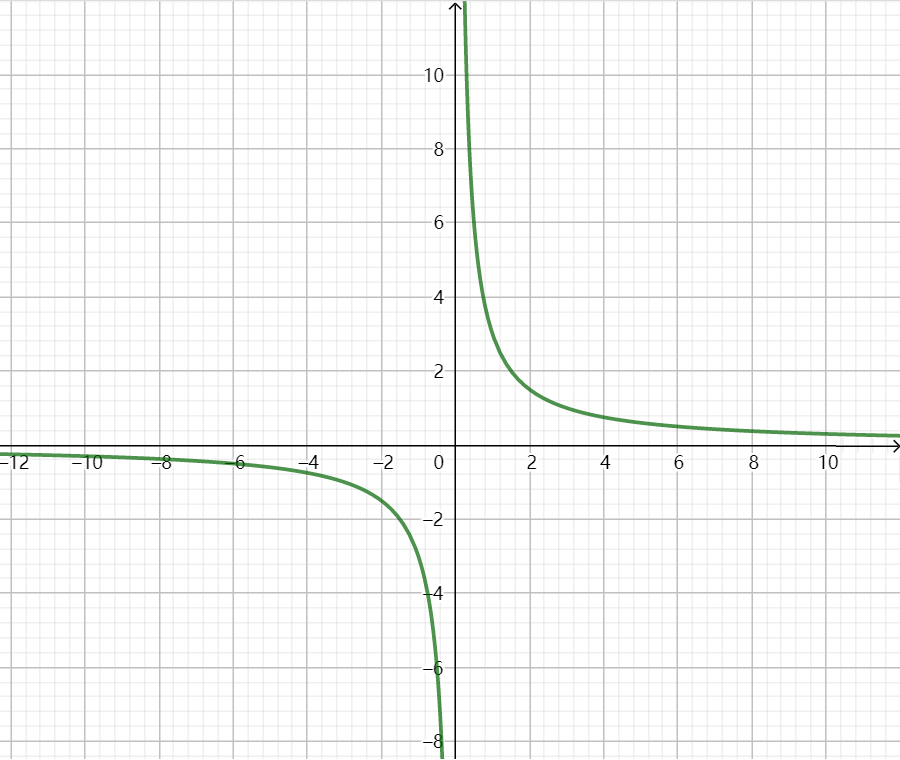
\includegraphics[width=0.6\textwidth]{tu/反比例函数1.png}
\end{wrapfigure}

我们说反比例函数的图像是一条曲线。右图中,第一象限中的部分叫做反比例函数的\textbf{正支},
它是函数在$x>0$时的图像;第三象限中的部分叫做反比例函数的\textbf{负支};它是函数在$x<0$时的图像。
$k>0$时,正支在第一象限,负支在第三象限;$k<0$时,正支在第四象限,负支在第二象限。

另外,反比例函数的图像关于原点中心对称。这可以通过性质:$f(-x) = -f(x)$得到。
对图像中每一点$(x, \,\,f(x))$,$(-x, \,\,-f(x)) = (-x, \,\,f(-x))$,因此它关于原点的对称点也在函数图像上。

对不同的$k$,反比例函数的图像有什么不一样呢?我们画出不同的$k$对应的反比例函数图像:

\begin{figure}[h] %this figure will be at the right
    % \vspace{-20pt}
    \centering
    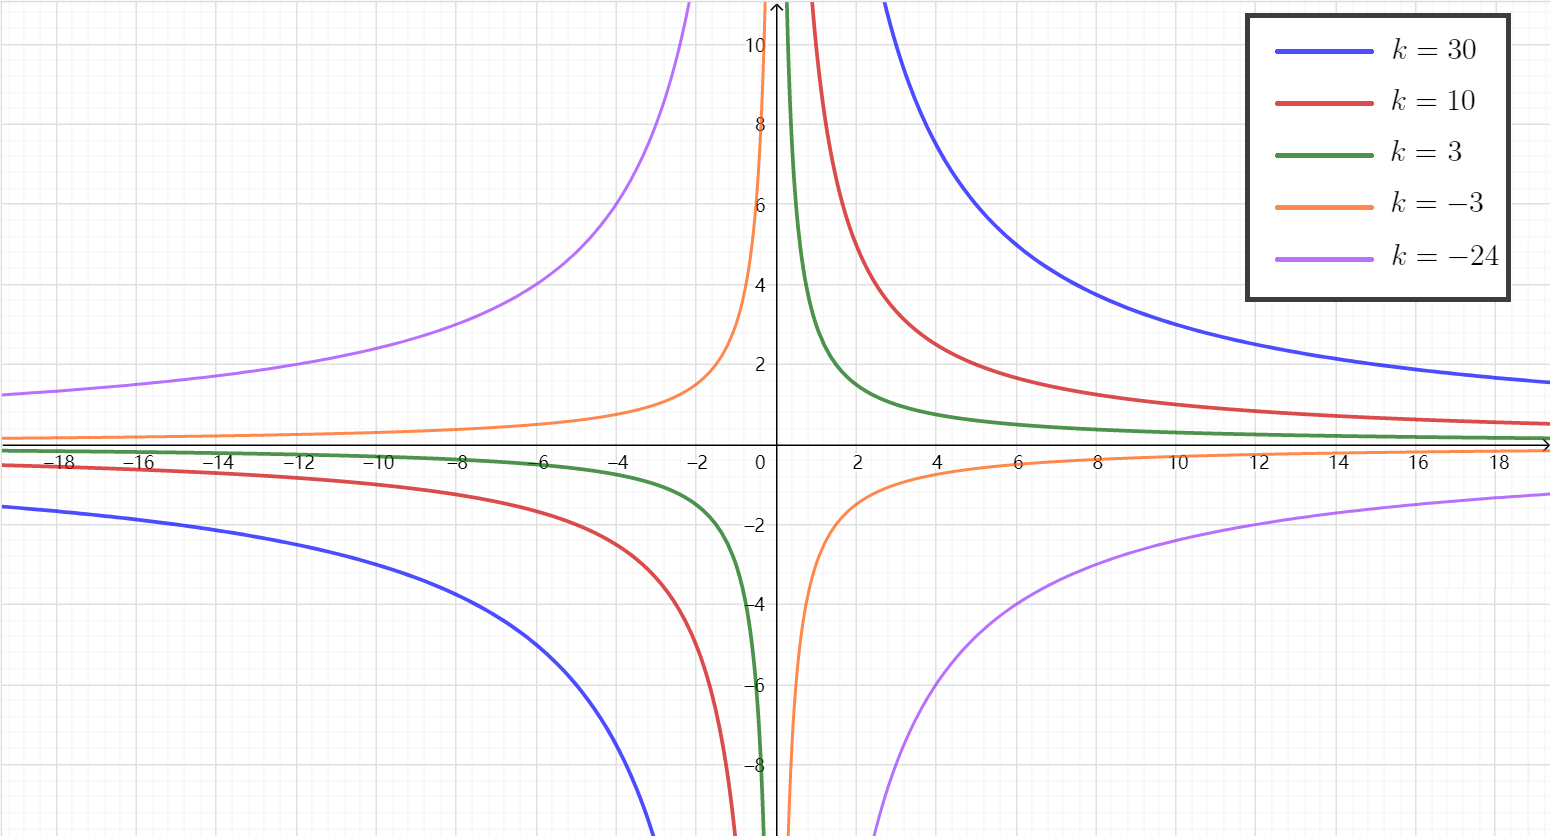
\includegraphics[width=0.9\textwidth]{tu/反比例函数2.png}
\end{figure}

首先,$k=3$的图像和$k=-3$的函数图像恰好关于$y$轴对称,也关于$x$轴对称。
一般来说,$k<0$时,函数图像和$-k$时的函数图像关于$y$轴和$x$轴对称。
由对称性,我们可以只研究$k>0$情况下函数图像的正支。

对比上图第一象限中三种颜色的曲线,我们可以发现,每条曲线都随着$x$变大而越来越平缓,
$x$越靠近$0$,曲线就越陡峭。观察不同曲线之间的区别,可以发现,$k$越大,曲线越“靠右上方”。
这并不难理解。比如,对横坐标$x = 4$来说,正数$k$越大,纵坐标$\frac{k}{4}$就越大,在图像中越“靠上”。
同样,要让纵坐标$f(x) = 4$,那么对应的横坐标$x = \frac{k}{4}$,于是正数$k$越大,$\frac{k}{4}$就越大,
在图像中越“靠右”。

反比例函数的图像还有一个基本性质:如果点$(a, \,\,b)$在图像上,那么$(b, \,\,a)$也在图像上。
这是因为$a = \frac{k}{b}$,当且仅当$b = \frac{k}{a}$。
\begin{xt}\label{xt:5-0-0}
    证明:\\
    \indent 1. 只要$(a, \,\,b)$在函数$x \mapsto \frac{k}{x}$的图像上,那么$(b, \,\,a)$、$(-a, \,\,-b)$、$(-b, \,\,-a)$
    都在图像上。\\
    \indent 2. 如果斜率为$-1$的直线$x\mapsto -x + c$和函数$ x \mapsto \frac{k}{x}$的图像有交点,
    那么$c^2 \geqslant 4k$。
\end{xt}

\section{二次函数}
一元一次式对应一次函数,而一元二次式对应着二次函数。一般来说,一元二次式可以写成$ax^2 + bx + c$的形式,
其中$a \neq 0$。我们把形如
$$ x \mapsto ax^2 + bx + c$$
的函数叫做二次函数。

我们从最简单的情形:$x\mapsto x^2$开始研究。下表是$x$取不同值时函数的值:

\begin{center}
    \begin{tabular}{| p{2em}<{\centering} | p{1.8em}<{\centering} | p{1.8em}<{\centering} | p{1.8em}<{\centering} | p{1.8em}<{\centering} | p{1.8em}<{\centering} | p{1.8em}<{\centering} | p{1.8em}<{\centering} | p{1.8em}<{\centering} | p{1.8em}<{\centering} |}
        \hline
        $x$ & -10 & -5 & -2 & -1 & 0 & 1 & 2 & 5 & 10 \\ [0.5ex] 
        \hline
        $f(x)$ & 100 & 25 & 4 & 1 & 0 & 1 & 4 & 25 & 100 \\   
        \hline
    \end{tabular}
\end{center}

首先可以发现,如果$a$和$b$是相反数,那么$f(a) = f(b)$。比如,$f(-5) = f(5)$、$f(-2) = f(2)$、
$f(-1) = f(1)$。这个性质可以写成:
$$ f(-x) = f(x).$$
这个性质可以用函数的定义证明:
$$ f(-x) = (-x)^2 = x^2 = f(x).$$

另外可以看到,$x<0$时,$f(x)$大于$0$,且$x$越大,$f(x)$越小,最终在$x=0$时函数值取$0$。
$x > 0$是,$f(x)$大于$0$,且$x$越大,$f(x)$越大。

函数$x\mapsto x^2$的图像是怎样的呢?和反比例函数情形一样:我们可以用描点法得到大致的模样,但目前我们掌握的知识,
还不足以严谨地勾画出它的图像。借助计算机作图软件,我们可以得到函数$x\mapsto x^2$的图像:

\begin{figure}[h] %this figure will be at the right
    \vspace{8pt}
    \centering
    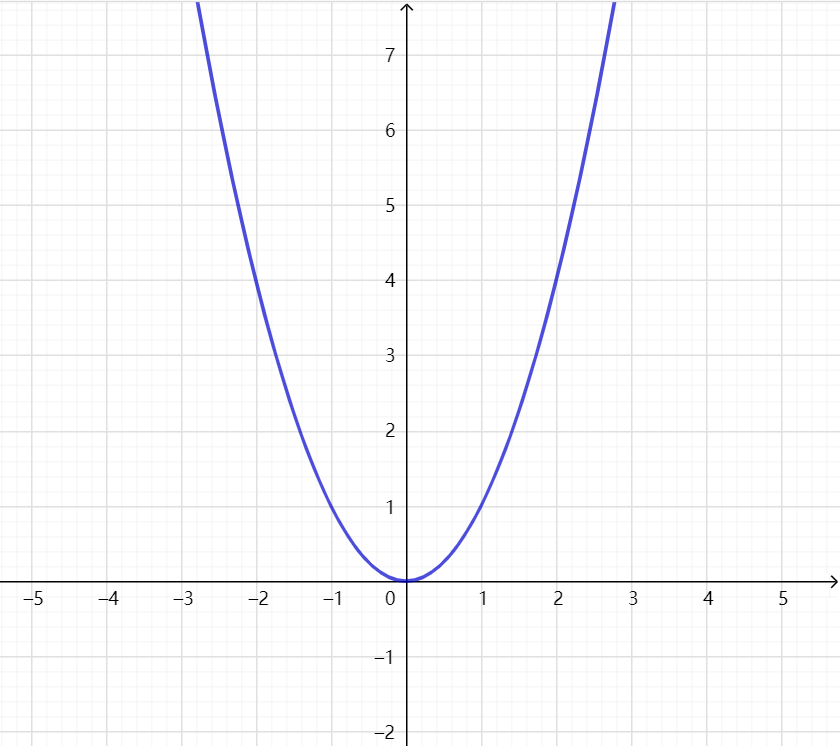
\includegraphics[width=0.6\textwidth]{tu/二次函数1.png}
\end{figure}

观察图像,这是一条曲线。首先可以注意到,它关于$y$轴对称。这一点可以用前面得到的性质证明。给定图像上一点:
$(x, \,\,x^2)$,$(-x, \,\,x^2)$也在图像上,所以图像关于$y$轴对称。由对称性,
我们可以先研究曲线在$x\geqslant 0$部分的性质。

可以发现,从$x=0$开始,随着$x$逐渐增大,函数值也逐渐增大,而且增长速度逐渐加快。
在$x=0$附近,曲线比较平缓,$x$增大后,曲线越来越陡峭。

如果把函数乘以系数$a$,得到$x\mapsto ax^2$,函数的性质会发生什么变化?
我们可以验证:$a > 0$时,以上提到的性质保持不变。$a < 0$时,函数的正负和增减性质颠倒了。
首先,$ax^2$总小于等于$0$。$x<0$时,$x$越大,函数值越大,$x>0$时,$x$越大,函数值越小。
从$x=0$开始,随着$x$逐渐增大,函数值逐渐减小,而且减小速度逐渐加快。
与$a>0$时相同的是:在$x=0$附近,曲线比较平缓,$x$增大后,曲线越来越陡峭。

\begin{figure}[h] %this figure will be at the right
    \vspace{8pt}
    \centering
    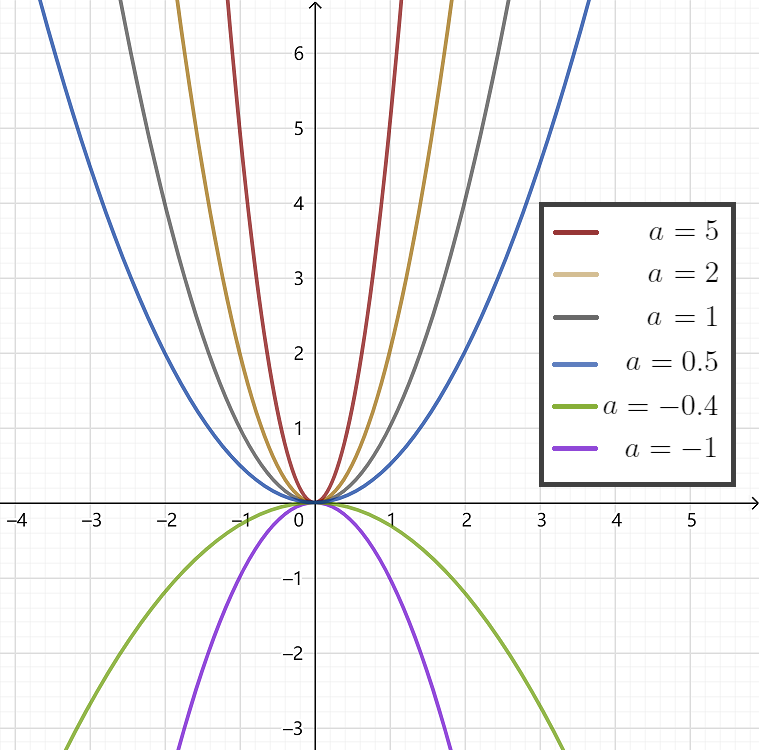
\includegraphics[width=0.5\textwidth]{tu/二次函数2.png}
\end{figure}

对于一般的一元二次式$ax^2+bx+c$,二次函数$x\mapsto ax^2+bx+c$的图像是怎样的呢?
上一章中,我们使用配方法解一元二次方程。用同样的方法,我们可以把$ax^2+bx+c$
写成:
\begin{align*}
    ax^2+bx+c &= a\left(x + \frac{b}{2a}\right)^2 + \frac{4ac - b^2}{4a}  \\
    &= a\left(x + \frac{b}{2a}\right)^2 - \frac{\Delta}{4a}. 
\end{align*}

因此,如果我们把$x\mapsto ax^2$的图像按$\left(-\frac{b}{2a}, \,\,-\frac{\Delta}{4a}\right)$平移,
就得到$x\mapsto ax^2+bx+c$的图像。
比如,要得到$x\mapsto 0.5x^2+0.8x-1$的图像,我们从
$x\mapsto 0.5x^2$出发。将$0.5x^2+0.8x-1$配方得到
$$ 0.5x^2+0.8x-1 = 0.5\left(x + 0.8\right)^2 - 1.32$$
于是将$x\mapsto 0.5x^2$按$(-0.8, \,\,-1.32)$平移,就得到$x\mapsto 0.5x^2+0.8x-1$的图像。

\begin{figure}[ht] %this figure will be at the right
    \centering
    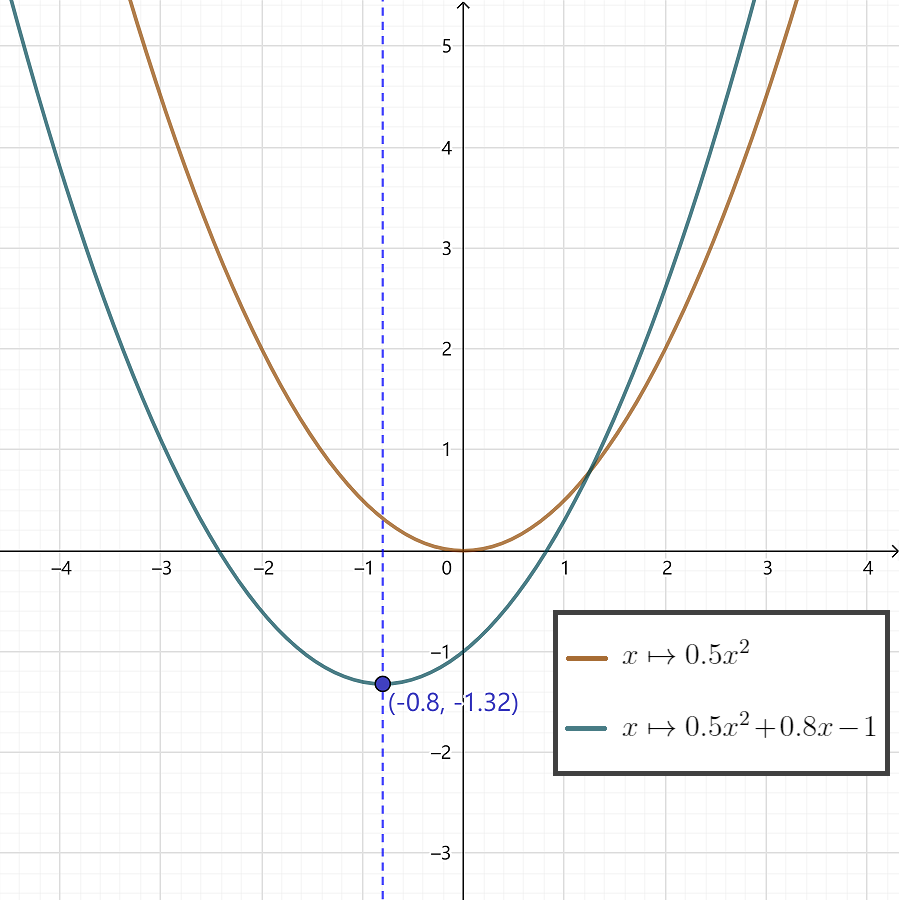
\includegraphics[width=0.45\textwidth]{tu/二次函数3.png}
\end{figure}

用$x\mapsto 0.5x^2+0.8x-1$作例子,可以看到,原来$x\mapsto ax^2$的图像关于$y$轴对称。
平移之后,图像关于直线$x = -\frac{b}{2a}$对称。$a>0$时,$x\mapsto ax^2$的图像最低点是$(0,\,\,0)$,
平移之后,最低点是$\left(-\frac{b}{2a}, \,\,-\frac{\Delta}{4a}\right)$。
$a<0$时,$x\mapsto ax^2$的图像最高点是$(0,\,\,0)$,
平移之后,最高点是$\left(-\frac{b}{2a}, \,\,-\frac{\Delta}{4a}\right)$。
直线$x = -\frac{b}{2a}$叫做二次函数图像的对称轴,
点$\left(-\frac{b}{2a}, \,\,-\frac{\Delta}{4a}\right)$叫做\textbf{二次函数图像的顶点}。
\begin{xt}\label{xt:5-1-0}
    \mbox{} \\    
    \indent 1. 二次函数$x\mapsto x^2$的图像和$x\mapsto ax + b$恰有一个交点,
    那么$a$、$b$满足怎样的关系?交点的坐标是多少?\\
    \indent 2. 二次函数$x\mapsto ax^2+bx+c$的图像和它关于点$(x_0, y_0)$平移后的图像有交点,
    则$(x_0, y_0)$应满足什么条件?交点个数可以是多少?
\end{xt}

\section{一元二次不等式}
通过研究二次函数的图像,我们可以直观地理解一元二次不等式。

一元二次不等式是类似$ax^2 + bx + c > 0$的不等式。其中的大于号也可以是小于号、大于等于号或小于等于号。
以不等式$ax^2 + bx + c > 0$来说,$x$是不等式的一个解,当且仅当点$(x, ax^2 + bx + c)$在$x$轴上方。
也就是说,$ax^2 + bx + c > 0$的解集,就是二次函数$ x \mapsto ax^2 + bx + c$在$x$轴上方的点的横坐标的集合。

观察$x \mapsto ax^2 + bx + c$的图像可知,如果$\Delta>0$,那么二次函数有两个零点。
$a>0$时,不等式的解集对应两个零点两侧的部分,是两个开区间的并集:
$$ (-\infty; \frac{-b - \Delta}{2a}) \cup (\frac{-b +\Delta}{2a}; \infty)$$
$a<0$时,不等式的解集对应两个零点之间的部分,即开区间:
$$ (\frac{-b - \Delta}{2a}; \frac{-b +\Delta}{2a}) $$
如果$\Delta<0$,那么二次函数没有零点。$a>0$时,二次函数的图像总在$x$轴上方,于是不等式的解集是全体实数。
$a<0$时,二次函数的图像总在$x$轴下方,于是不等式的解集是空集。

如果$\Delta = 0$,那么二次函数恰有一个零点。
$a>0$时,不等式的解集对应零点两侧的部分,是两个开区间的并集:
$$ (-\infty; \frac{-b}{2a}) \cup (\frac{-b}{2a}; \infty)$$
$a<0$时,二次函数的值不大于零,于是不等式的解集是空集。

要是不等式的大于号换成大于等于号,则相关的“开”的部分也换成“闭”。如果$\Delta>0$,二次函数有两个零点。
$a>0$时,不等式$ax^2 + bx + c \geqslant 0$的解集是:
$$ (-\infty; \frac{-b - \Delta}{2a}\,] \cup [\,\frac{-b +\Delta}{2a}; \infty)$$
$a<0$时,不等式的解集是:
$$ [\,\frac{-b - \Delta}{2a}; \frac{-b +\Delta}{2a}\,] $$
如果$\Delta<0$,那么二次函数没有零点。$a>0$时,二次函数的图像总在$x$轴上方,于是不等式的解集是全体实数。
$a<0$时,二次函数的图像总在$x$轴下方,于是不等式的解集是空集。

如果$\Delta = 0$,那么二次函数恰有一个零点。
$a>0$时,不等式的解集包括了零点,因此是全体实数。
$a<0$时,二次函数的值不大于零,于是不等式的解集是单元集:$\{\frac{-b}{2a}\}$。

要是不等式的大于号(大于等于号)换成小于号(小于等于号),只需要把左边的项移到右边,
就转化成大于号(大于等于号)的情况。

\begin{ex}
    \mbox{}\\
    \indent 1. 求不等式$2x^2 - 5x + 2 > 0$的解集。\\
    \indent 2. 求不等式$x^2 - 6x + 9 \geqslant 0$的解集。
\end{ex}
\begin{so}
    \mbox{}\\
    \indent 1. 首先求一元二次方程$2x^2 - 5x + 2 = 0$的解。依公式可得:
    $$ x_1 = 0.5, \quad x_2 = 2.$$
    因此,不等式的解集是$(-\infty; 0.5) \cup (2; \infty)$。\\
    \indent 2. 首先求一元二次方程$x^2 - 6x + 9 = 0$的解。依公式可得:
    $$ x = 3.$$
    因此,不等式的解集是全体实数。
\end{so}

一元二次不等式还可以用来解反比例函数和一次函数的不等式。
\begin{ex}
    求不等式$\frac{8}{x} > x + 2$的解集。
\end{ex}
可以把这个不等式理解为反比例函数$x \mapsto \frac{8}{x}$和一次函数$x \mapsto x + 2$的图像的关系。
$x$是不等式$\frac{8}{x} > x + 2$的一个解,当且仅当点$(x, \frac{8}{x})$在点$(x, \,\,x + 2)$上方。
如果我们画出两个函数的图像,并找到反比例函数在$x \mapsto \frac{8}{x}$在一次函数$x \mapsto x + 2$
图像上方的部分,那么这部分的点的横坐标,就是不等式的解。

观察两者图像可知,解集大致对应第三象限中曲线和直线交点左侧的部分,以及第一象限中曲线和直线交点左侧的部分。
具体交点的位置,我们可以通过解方程$\frac{8}{x} = x + 2$得到。而这个方程可以转化为一元二次方程。

\begin{figure}[h]
    \vspace{4pt}
    \centering
    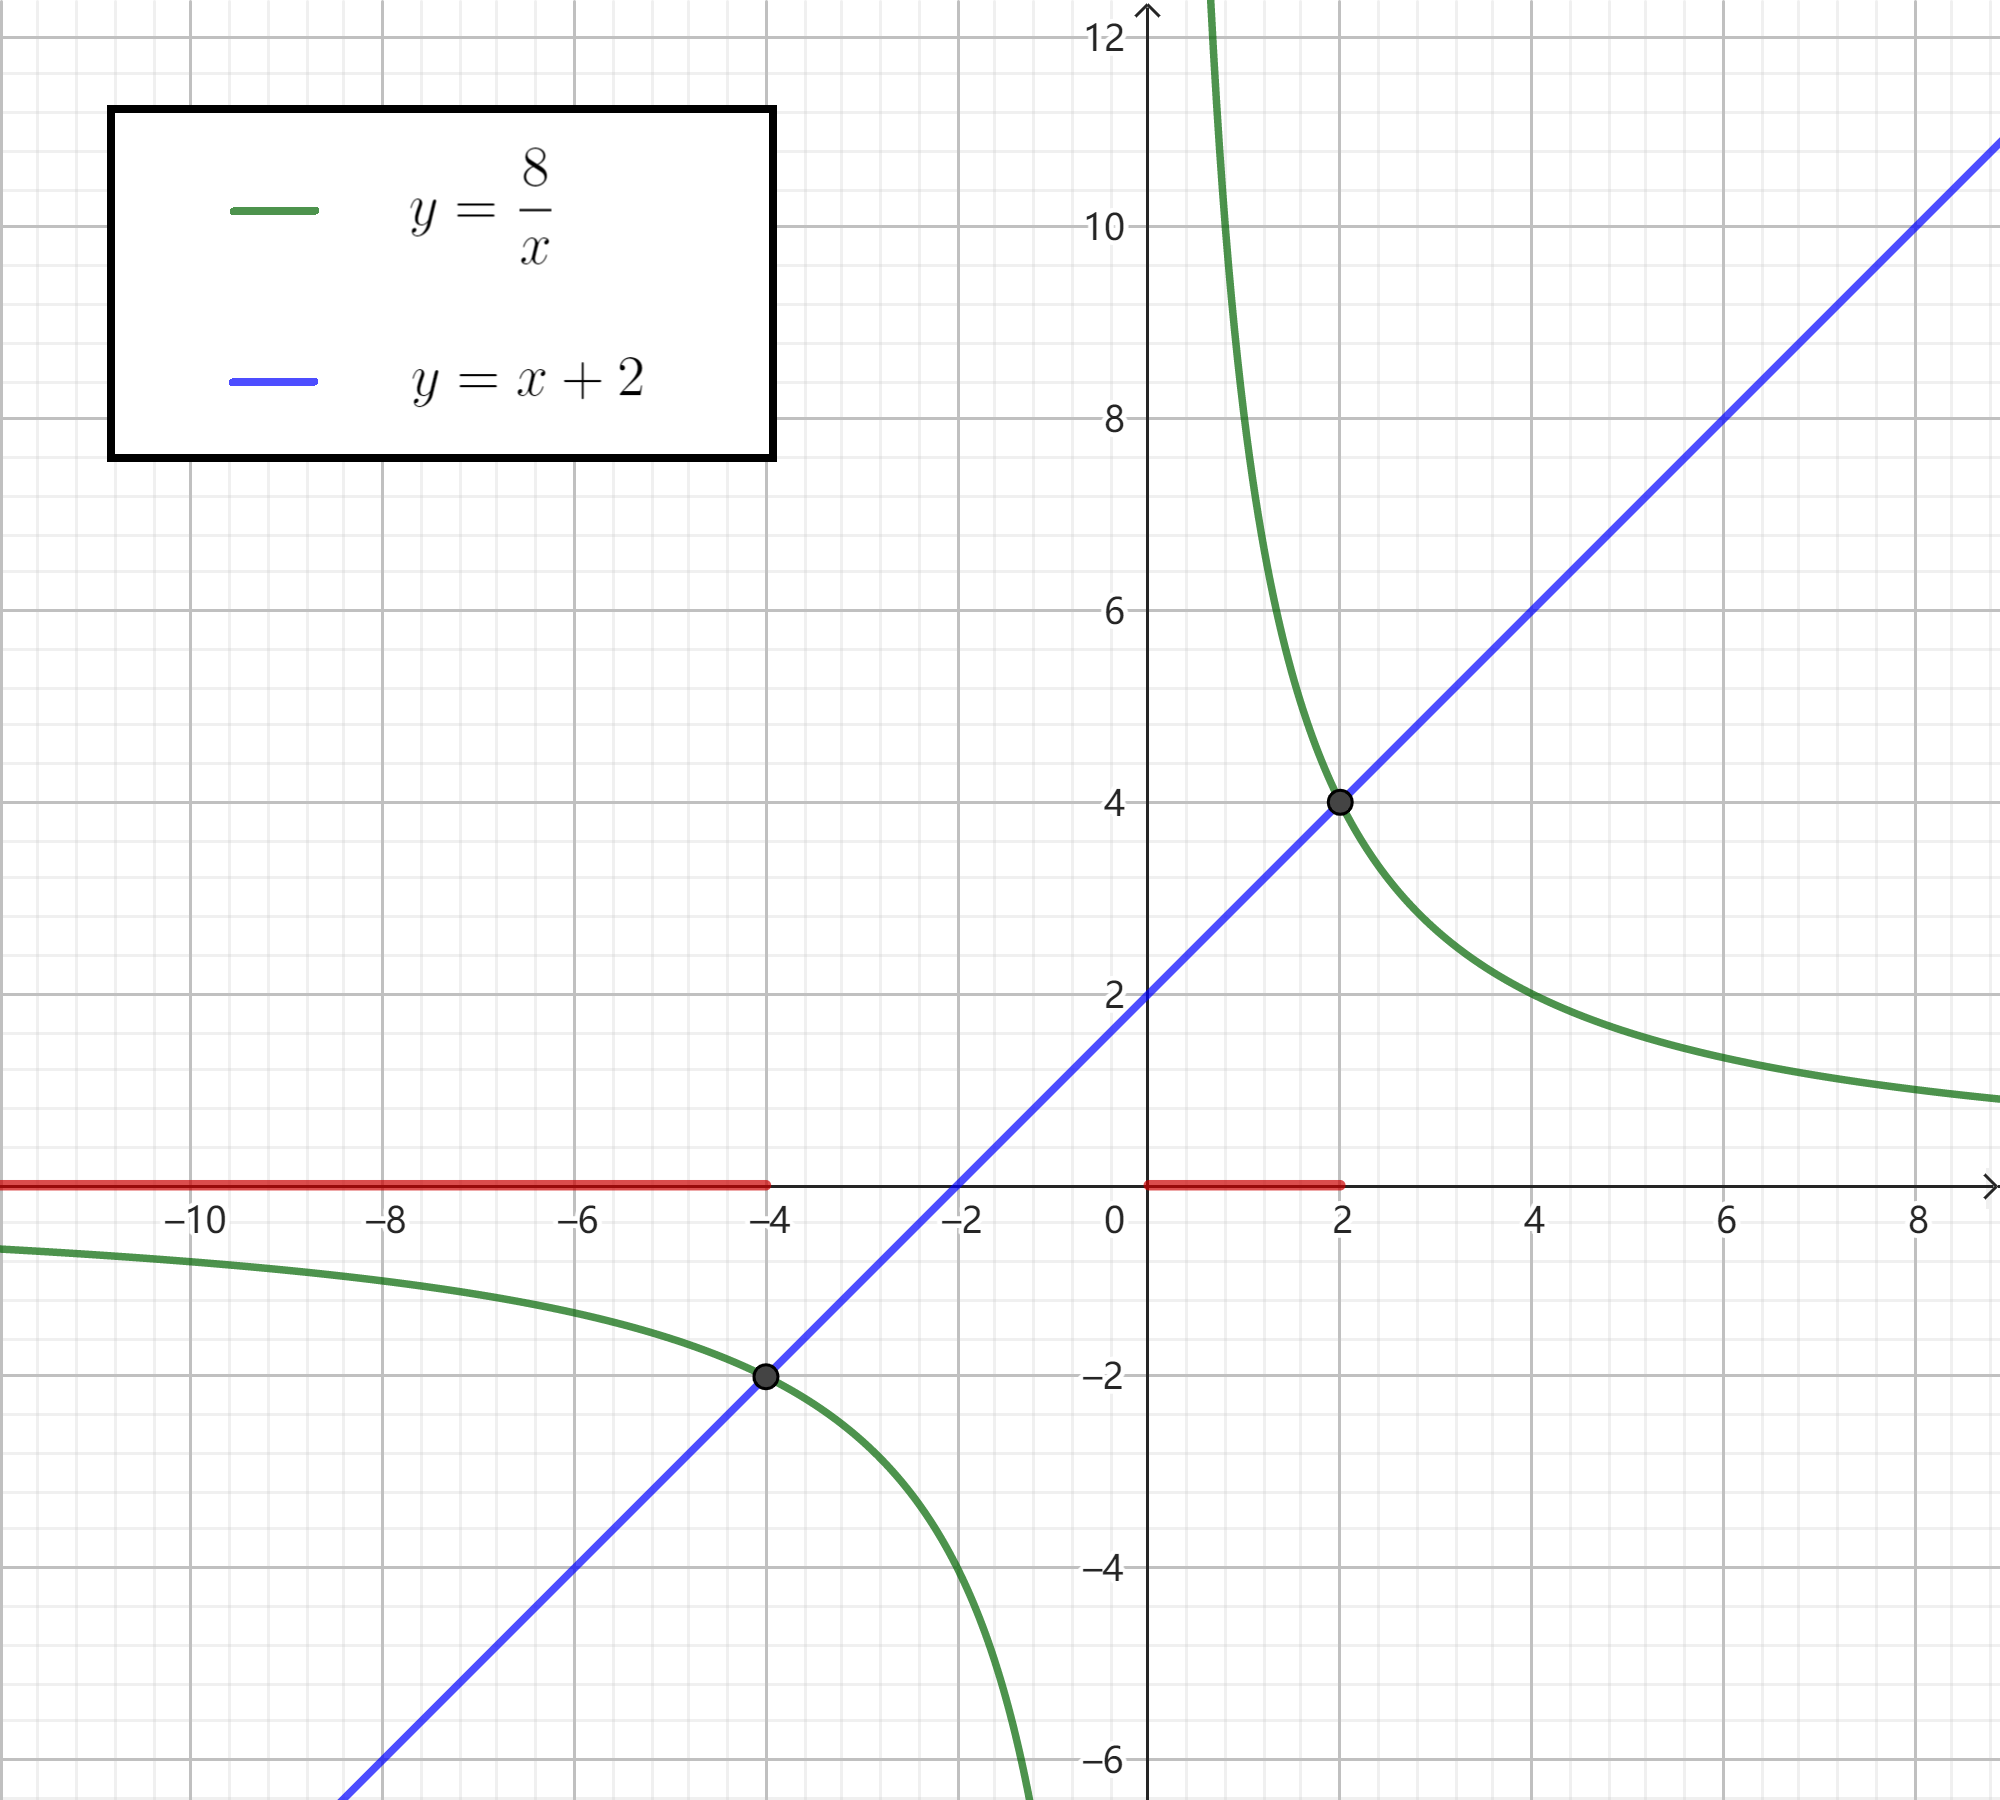
\includegraphics[width=0.5\textwidth]{tu/一元二次不等式1.png}
\end{figure}

把$\frac{8}{x} = x + 2$两边乘以$x$,再把常数项$8$移到右边,就得到方程:
$$ 0 =  x^2 + 2x - 8.$$
这是一个一元二次方程,解为:
$$ x_1 = -4, \quad x_2 = 2$$
它们分别对应点$(-4, \,\,-2)$和$(2, \,\,4)$(注意不是$(-4, \,\,0)$和$(2, \,\,0)$)。这两个点就是第三、第一象限中曲线和直线交点的位置。
因此,我们可以得出结论:不等式的解集是$(-\infty; -4) \cup (0; 2)$。

\begin{xt}\label{xt:5-2-0}
    解以下不等式:\\
    \indent 1. $3x^2 - 8x + 4 < 0$ \\
    \indent 2. $2x^2 + 8x + 9 \geqslant 7x + 10$ \\
    \indent 3. $\frac{2}{x} < 6x- 7$ 
\end{xt}




\end{document}